\documentclass{article}

%% Language and font encodings
\usepackage[english]{babel}

%% Sets page size and margins
\usepackage[margin=1in]{geometry}

%% Useful packages
\usepackage{amsmath}
\usepackage{bm}
\usepackage{graphicx}
\usepackage{mathtools}
\usepackage{wrapfig}

%% Change to another style
\newcommand{\MatrixVariable}[1]{\bm{\mathit{#1}}}

\title{ELE 381/COS 381 Review Sheet}
\author{Akash Levy}

\begin{document}
\maketitle

\section{What makes CDMA work for my smartphone?}

\subsection{Cellular network structure}

\begin{wrapfigure}[12]{r}[0.5in]{0.275\textwidth}
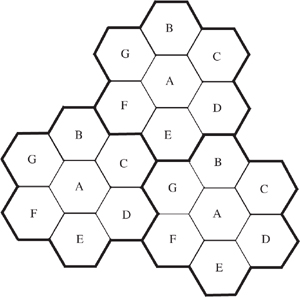
\includegraphics[width=\linewidth]{freq_reuse.png}
\end{wrapfigure}

The cells of a cellular network provide a convenient way of representing the deployment space. Each cell represents a fragment of two-dimensional physical space within which signals are transmitted. \\
\\
Each cell has one \textbf{base station} (i.e. a cell tower) and many \textbf{mobile stations} (i.e. mobile devices). \\
\\
Different cells operate on different frequencies. The frequencies can be reused once the signal has degraded over a long enough distance. \\
\\
The number of different frequencies defines the \textbf{frequency reuse factor}. For the figure on the right, this factor is 7. \\

\subsection{Techniques for multiple access}

\subsubsection{Frequency Division Multiple Access (FDMA)}

\textit{Users are assigned frequency bands and can transmit simultaneously} \\
There is no interference since the different frequencies are orthogonal to one another. This technique involves subdividing the different frequencies used in the cells.

\subsubsection{Time Division Multiple Access (TDMA)}

\textit{Users are assigned time slots and take turns} \\
There is no interference since no two devices transmit at the same time.

\subsubsection{Code Division Multiple Access (CDMA)}

\textit{Users are assigned different codes and can transmit simultaneously in the same frequency band} \\
All users can transmit at the same time on one frequency band using different codes. By XORing the signal bits by user's unique code, information can be transmitted in such a way that only the user's signal looks non-random. But now interference becomes an issue since there is no orthogonality in the actual signals, only in the codes. \\
CDMA is widely used in 3G networks.

\subsubsection{Orthogonal Frequency Division Multiplexing (OFDM)}

\textit{Divide transmission in both time and frequency domains} \\
This can help minimize interference between different frequencies. OFDM is used in 4G/LTE networks. \\

\subsection{Distributed Power Control (DPC)}

In order to solve the interference problem with CDMA, we want to minimize the transmission powers while achieving some target \textbf{Signal to Interference Ratio (SIR)} for each link. DPC is a fully distributed algorithm that uses proportional error feedback to enable convergence of the SIRs to the target values.

\subsubsection{Symbols for Equations}

$N$: number of transmitters and receivers \\
$p_i$: transmit power of link $i$ \\
$G_{ij}$: \textbf{channel gain} between transmitter $i$ and receiver $j$ \\
$G_{ii}$: \textbf{direct channel gain} \\
$d_{ij}$: distance between transmitter $i$ and receiver $j$ \\
$\alpha$: distance drop-off power (ideally 2, typically between 2 and 4) \\
$\gamma_i$: target SIR for link $i$ \\
$\MatrixVariable{D}$: diagonal matrix with $\gamma_i$ as the diagonal entries \\
$\MatrixVariable{F}$: matrix capturing given channel conditions (see corresponding equation in section below) \\
$\rho(\MatrixVariable{DF})$: the largest eigenvalue of the matrix $\MatrixVariable{DF}$

\subsubsection{Equations}

Channel gain drops off as an inverse power of the distance between transmitter and receiver:
$$G_{ij} \propto d_{ij}^{-\alpha}$$
SIR is defined as ratio of channel power ($G_{ii}p_i$) to noise (sum of all other channel powers plus channel noise):
$$\text{SIR}_i = \frac{G_{ii}p_i}{\sum_{i \neq j} G_{ij}p_j + n_i}$$
Proportional error feedback for SIR:
$$p_i\lbrack t+1 \rbrack = \frac{\gamma_i}{\text{SIR}_i \lbrack t \rbrack} p_i \lbrack t \rbrack$$
$\MatrixVariable{F}$ matrix capturing given channel conditions:
$$F_{ij} = G_{ij}/G_{ii}$$
If $\rho(\MatrixVariable{DF}) < 1$, target SIRs can be achieved simultaneously (i.e. DPC problem is feasible)

\subsection{Possible question types}

\begin{enumerate}
\item Given coordinates of transmitters/receivers $(x_i, y_i)$, construct the $\MatrixVariable{G}$ matrix for an $\alpha$ value of 2 (up to a constant). \\
\textit{Answer: distance $d_{ij}$ is given by $\sqrt{(x_i-x_j)^2+(y_i-y_j)^2}$, then use $G_{ij} = (Constant)*d_{ij}^{-\alpha}$}
\item Given $\MatrixVariable{G}$ matrix and initial values for $\vec p$, $\vec n$, $\vec \gamma$, compute SIRs for each link and $\vec p$ for the next step. \\
\textit{Answer: use $\text{SIR}_i = \frac{G_{ii}p_i}{\sum_{i \neq j} G_{ij}p_j + n_i}$ and $p_i\lbrack t+1 \rbrack = \frac{\gamma_i}{\text{SIR}_i \lbrack t \rbrack} p_i \lbrack t \rbrack$}
\item Given a 2x2 $\MatrixVariable{G}$ matrix and $\vec \gamma$, determine whether or not the DPC problem is feasible. \\
\textit{Answer: D just has $\gamma_i$ as diagonal elements, $F_{ij} = G_{ij}/G_{ii}$, then eigenvalues can be computed using the quadratic equation. Finally, check that $\rho(\MatrixVariable{DF}) < 1$}
\end{enumerate}

\clearpage

\section{How does Google sell ad spaces?}

\subsection{Types of auctions}

\begin{wrapfigure}[11]{r}[0.5in]{0.4\textwidth}
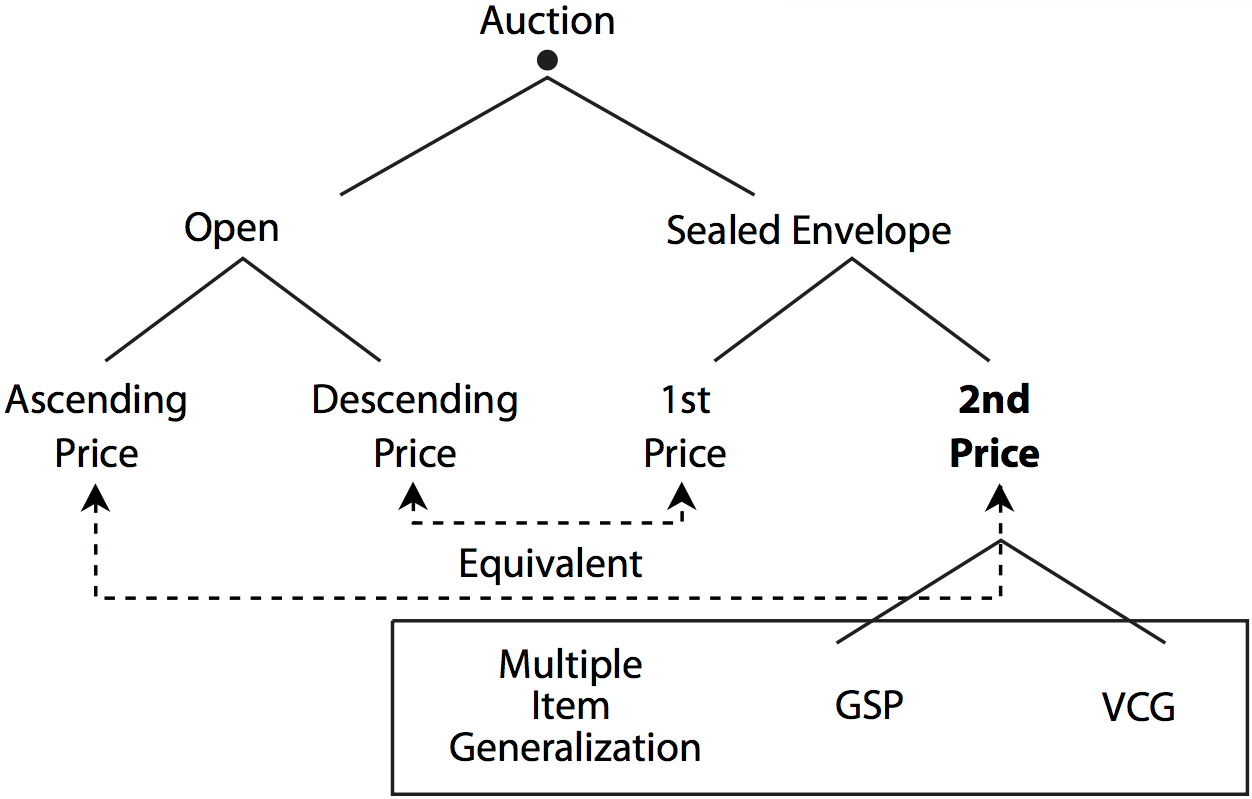
\includegraphics[width=\linewidth]{auctions.png}
\end{wrapfigure}

\textbf{Ascending price auction:} base price followed by bids that increase, highest bidder wins \\
\textbf{Descending price auction:} ceiling price that is lowered until someone agrees to price, first bidder wins \\
\textbf{Sealed envelope auction:} everyone bids without knowing what others bid, highest bidder wins \\

\subsection{Types of sealed envelope auctions}

\textbf{First price auction:} highest bidder pays own bid, must shade valuation to have positive payoff \\
\textbf{Second price auction:} highest bidder pays second highest bidder's bid, bidding valuation is optimal \\
\textbf{Generalized second price (GSP) auction:} for multiple items, highest bidder pays second highest bidder's bid, second highest bidder pays third highest bidder's bid etc.; bidding valuation may not be optimal \\
\textbf{Vickrey-Clark-Groves (VCG) auction:} for multiple items, highest bidder is charged for how much the win reduces the payoffs of the other bidders; bidding valuation is optimal \\
\\
Additionally, ad space sellers can have a \textbf{reserve price} to increase their own profit. This involves having a minimum price below which no sale is made. \\

\subsection{Stopping problem}
Don’t hire the first $n/e$ candidates \\
Hire the first candidate that's better than all the ones you've seen so far \\
$\text{Prob}(success) = 1/e$ \\

\subsection{Variables}

$N$: number of bidders, \ \ $K$: number of items being bid on \\
$C_i$: clickthrough rate for bidder $i$, \ \ $R_i$: revenue per click for bidder $i$ \\
$b_i$: bid of bidder $i$, \ \ $p_i$: price bidder $i$ has to pay, \ \  $v_i$: valuation of bidder $i$ where $v_i = C_iR_i$ \\
$U_i$: payoff function of bidder $i$ (i.e. profit) \\

\subsection{Possible question types}

\begin{enumerate}
\item Given $\vec C$ and $\vec R$, compute the valuation of each bidder. \\
\textit{Answer: use $v_i = C_iR_i$}
\item Explain why a first price auction is equivalent to a descending price auction and why a second price auction is equivalent to an ascending price auction. What will be the outcome in each case; will there be a difference in the amount paid by the highest bidder? \\
\textit{Answer: In a descending price auction, the auction ends as soon as the first bid is made. So when the price reaches the second highest bidder's valuation, the highest bidder will bid. In an ascending price auction, the auction ends when no more bids are made. Thus the highest bidder need only bid marginally higher than the second highest bidder's bid in the end. This value will be close to the second highest bidder's valuation. So the outcome will be the same in either case.}
\item Given [first/second/GSP/VCG] auction and $v_i$ for each bidder $i$, sketch the payoff and compute the optimal bid of bidder 1 assuming the others bid [their valuation/the valuation of the next highest bidder]. \\
\textit{Answer: compute the piece-wise $U_1(b_1)$ by considering who would win in each scenario, then plot and discover maximum value of $U_1(b_1)$}
\item Suppose you wanted to hire a candidate from a pool of 27 candidates but you must hire them on the spot. After which candidate should you stop? \\
\textit{Answer: $n/e \approx 27/2.7 = 10$} \\
\end{enumerate}

\section{How does Google rank webpages?}

\subsection{Factors involved in ranking}

\begin{wrapfigure}[9]{r}[0.5in]{0.275\textwidth}
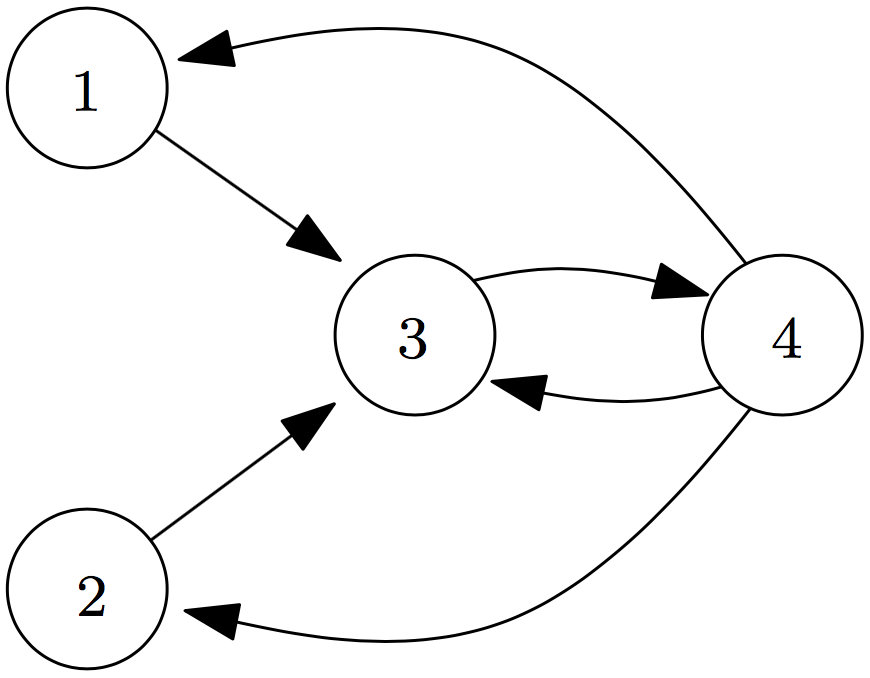
\includegraphics[width=\linewidth]{web_graph.png}
\end{wrapfigure}

\textbf{Relevance score:} how relevant a page is to a given query
\\
\textbf{Importance score:} how important a page is relative to other pages \\
\\
\textbf{PageRank} treats web browsing as a random walk on the link graph and can be studied as a \textbf{Markov chain} in probability theory. \\

\subsection{Variables}

$N$: total number of nodes \\
$O_i$: out-degree of node $i$ \\
$\MatrixVariable{w}$: dangling node indicator vector ($i$th entry is 1 if webpage is dangling node, 0 otherwise) \\
$\pi \lbrack k \rbrack$: importance vector at iteration $k$ \\
$\pi^*$: represents the stationary distribution of the Markov chain whose transition probabilities are in \MatrixVariable{G}, is the left eigenvector corresponding to the dominant eigenvalue of \MatrixVariable{G}, and the importance vector as $k \to \infty$ \\
$\MatrixVariable{H}$: normalized adjacency matrix, whose $(i,j)$th entry is $1/O_i$ if link exists from webpage $i$ to $j$, 0 otherwise \\
$\hat{\MatrixVariable{H}}$: $\MatrixVariable{H}$, but accounting for dangling nodes by making them equally likely to navigate to every other page \\
$\theta$: random teleportation factor, $1-\theta$ is the probability that teleportation occurs; controls the trade-off between convergence speed and relevance of graph in computing importance  \\
$\MatrixVariable{G}$: the Google matrix, which is $\MatrixVariable{H}$ with teleportation \\
$\MatrixVariable{v}$: an arbitrary probability distribution for linking to each page \\
$\MatrixVariable{A}$: adjacency matrix, whose $(i,j)$th entry is 1 if link exists from webpage $i$ to $j$, 0 otherwise \\

\subsection{Equations}

When running PageRank iteratively, the update equation is:
$$\pi^T \lbrack k \rbrack = \pi^T \lbrack k-1 \rbrack \MatrixVariable{H}$$
Or alternatively:
$$\pi \lbrack k \rbrack = \MatrixVariable{H}^T \pi \lbrack k-1 \rbrack$$
As $k \to \infty$:
$$\lim_{k \to \infty}\pi[k] = \pi^*$$
To solve the dangling node problem, we can modify H as follows:
$$\hat{\MatrixVariable{H}} = \MatrixVariable{H} + \frac{1}{N}(\MatrixVariable{w}\MatrixVariable{1}^T) $$
To ensure that there is a unique solution, we use teleportation in the Google matrix:
$$\MatrixVariable{G} = \theta \hat{\MatrixVariable{H}} + (1-\theta) \frac{1}{N}\MatrixVariable{1}\MatrixVariable{1}^T$$
If we compute the left eigenvector of $\MatrixVariable{G}$, we find that it gives us $\pi^*$:
$$\pi^{*T} = \pi^{*T} \MatrixVariable{G}$$
Or alternatively:
$$\pi^* = \MatrixVariable{G}^T \pi^*$$
We can generalize the G matrix to use an arbitrary probability distribution instead of equal weighting. We do this for both the dangling vector component and the teleportation component. We then get:
$$\MatrixVariable{G} = \theta \MatrixVariable{H} + (\theta \MatrixVariable{w} + (1-\theta)\MatrixVariable{1})\MatrixVariable{v}^T$$
Dangling nodes are only visited with a probability of $(1-\theta)/N$. In a symmetric graph, you find that the symmetric nodes have equal importance. \\
\\
The eigenvalues of \MatrixVariable{G} have the following property:
$$1 = \lambda_1 > |\lambda_2| \geq |\lambda_3| \geq |\lambda_4| \geq ...$$
The convergence speed is governed by the magnitude of the second-largest eigenvalue $\lambda_2$, which is close to $\theta$. \\
\\
For the \textbf{Kleinberg HITS algorithm}: \\
The authority vector is the right eigenvector of $\MatrixVariable{A}^T\MatrixVariable{A}$ corresponding to its largest eigenvalue. \\
The hub vector is the right eigenvector of $\MatrixVariable{A}\MatrixVariable{A}^T$ corresponding to its largest eigenvalue. \\

\subsection{Possible question types}

\begin{enumerate}
\item Given a link graph, compute $\MatrixVariable{H}$ and $\MatrixVariable{G}$ for given $\theta$. \\
\textit{Answer: determine the adjacency matrix, normalize by row for $\MatrixVariable{H}$, then compute $\MatrixVariable{G}$ using the formula $\MatrixVariable{G} = \theta \MatrixVariable{H} + (1-\theta) \frac{1}{N}\MatrixVariable{1}\MatrixVariable{1}^T$}
\item Given ($\MatrixVariable{H}$/$\hat{\MatrixVariable{H}}$/$\MatrixVariable{G}$) and $\pi \lbrack 0 \rbrack$, compute $\pi \lbrack 1 \rbrack$ and $\pi \lbrack 2 \rbrack$. \\
\textit{Answer: use the PageRank update equation}
\item Given a symmetric graph (possibly containing dangling nodes), compute $\pi^*$. \\
\textit{Answer: use fact that dangling nodes are only visited with probability $(1-\theta)/N$ and nodes which can be interchanged have equal probability}
\item Given some arbitrary normalized initial vector $\pi \lbrack 0 \rbrack$ and $\MatrixVariable{G}^T$ in its diagonalized form, compute $(\MatrixVariable{G}^T)^\infty \pi \lbrack 0 \rbrack$. \\
\textit{Answer: ignore the initial vector $\pi \lbrack 0 \rbrack$ and just take the eigenvector of $\MatrixVariable{G}^T$ corresponding to eigenvalue $\lambda_1=1$ (this will be the column of the diagonalizing matrix with corresponding diagonal entry 1)}
\item Given a symmetric graph (possibly containing dangling nodes), how would the importance change if a link were added/removed to produce another symmetric graph? \\
\textit{Answer: use the fact that the graph is symmetric in both cases to construct a simple set of linear equations for the new graph}
\item How would you solicit and aggregate feedback from individual users to enable personalized ranking? \\
\textit{Answer: open-ended, but can talk about how user behavior could define $\MatrixVariable{v}$ based on how likely a user was in the past to click on links of a certain type}
\end{enumerate}

\section{How does Netflix recommend movies?}

\subsection{Types of recommendation systems}

\textbf{Content-based:} recommendations given on the basis of purchases and browsing history \\
\textbf{Collaborative:} recommendations given on the basis of what similar users liked \\
\\
The success of these recommendation algorithms can be measured with the \textbf{Root Mean Squared Error (RMSE)}: \\
$$\text{RMSE} = \sqrt{\sum_{(u,i)} \frac{(r_{ui} - \hat{r}_{ui})^2}{C}}$$ \\

\subsection{Variables}

$\bar{r}$: average over all ratings \\
$b_u$: user bias to take into account user behavior \\
$b_i$: movie bias to take into account quality of different movies \\
$r_{ui}$: the rating of user $u$ for movie $i$ \\
$\hat{r}_{ui}$: baseline predictor (see equations below) \\
$\lambda$: the weighting for \textbf{regularization} (which involves adding a weighted sum of biases into the problem) \\
$\MatrixVariable{R}$: ratings matrix in the form $r_{ui}$ \\
$\MatrixVariable{\hat{R}}$: baseline predictor matrix with entry $u,i$ in the form $\hat{r}_{ui}$ \\
$\MatrixVariable{\tilde{R}}$: final error matrix after least-squares \\
$\MatrixVariable{\tilde{R}^N}$: final error matrix after least-squares and neighborhood method \\
$d_{ij}$: movie-movie similarity \\
$d_{uv}$: user-user similarity \\
$L$: neighborhood size (how many neighbors to pick) \\
$\mathcal{L}_i$: top L neighbors to a given movie/user (movie/user cannot be own neighbor) \\
$\hat{r}_{ui}^N$: the baseline predictor with the neighborhood method ``N" (see equations below) \\
$\MatrixVariable{A}$: a matrix with a 1 in column $u$ (or $i$) and 0s elsewhere \\
$\MatrixVariable{c}$: a vector with entries $r_{ui} - \bar{r}$ \\

\subsection{Equations}

The equation for the baseline predictor is:
$$\hat{r}_{ui} = \bar{r} + b_u + b_i$$
To get the biases:
$$\text{minimize}_{\lbrace b_u,b_i \rbrace} \sum_{(u,i)} (r_{ui} - \hat{r}_{ui})^2$$
This problem can be solved with least-squares. The matrix equation for solving least-squares is:
$$(\MatrixVariable{A}^T\MatrixVariable{A})\MatrixVariable{b} = \MatrixVariable{A}^T\MatrixVariable{c}$$
Remove the biases by subtracting the baseline predictor from the existing ratings:
$$\tilde{\MatrixVariable{R}} = \MatrixVariable{R} - \hat{\MatrixVariable{R}}$$
$$\tilde{r}_{ui} = 0 \text{ if no rating available by user}$$
Movie-movie similarity can be computed with cosine similarity:
$$d_{ij} = \frac{\MatrixVariable{r}_i \cdot \MatrixVariable{r}_j}{|\MatrixVariable{r}_i||\MatrixVariable{r}_j|} = \frac{\sum_u \tilde{r}_{ui} \tilde{r}_{uj}}{\sqrt{\sum_u (\tilde{r}_{ui})^2 \sum_u (\tilde{r}_{uj})^2}} = \text{cos}(\theta_{\MatrixVariable{r}_i,\MatrixVariable{r}_j}) $$
Note: the sum is only taken over movies which both users have rated. If none exist, $d_{ij} = 0$. \\
The new predictor is then:
$$\hat{r}_{ui}^N = \hat{r}_{ui} + \frac{\sum_{j \in \mathcal{L}_i} d_{ij} \tilde{r}_{uj}}{\sum_{j \in \mathcal{L}_i} |d_{ij}|} = \bar{r} + b_u + b_i + \frac{\sum_{j \in \mathcal{L}_i} d_{ij} \tilde{r}_{uj}}{\sum_{j \in \mathcal{L}_i} |d_{ij}|}$$
An analogous result holds with the above two equations for user-user similarity (just replace $i$ with $u$ and $j$ with $v$). \\

\subsection{Latent factors}
In the latent factors method, each user has some parameters $p[0,u]$, $p[1,u]$, ... and each movie has some parameters $q[0,i]$, $q[1,i]$, ... Then the prediction is:
$$\text{prediction}[u,i] = \MatrixVariable{p} \cdot \MatrixVariable{q} = p[0,u]*q[0,i] + p[1,u]*q[1,i] + ...$$
If you have latent factor matrices $\MatrixVariable{P}$ and $\MatrixVariable{Q}$, then $\MatrixVariable{P}\MatrixVariable{Q}^T$ gives you the prediction matrix. \\
You can then optimize by holding $\MatrixVariable{p}$ fixed and optimizing $\MatrixVariable{q}$, then alternating. \\

\subsection{Possible question types}

\begin{enumerate}
\item Given some ratings, compute $\bar{r}$. \\
\textit{Answer: compute the average of all the ratings}
\item Given some ratings and some predictions, compute the RMSE with $C = 1$. \\
\textit{Answer: take the sum over the square errors of each prediction and square root it}
\item Suppose we take the biases to be the average deviation from $\bar{r}$ of the movie's/user's ratings. Compute the biases $b_u$ and $b_i$ for a given set of ratings. Why is this technique for computing biases not generally used in real recommendation systems? \\
\textit{Answer: compute the average rating for each movie/user, take the difference between the rating and the average rating over all movies, use those differences as the biases $b_u$ and $b_i$; this technique is generally not used because it does not necessarily give biases that minimize the RMSE}
\item Given some ratings, compute the movie-movie similarities. Which movie is movie X most similar to? \\
\textit{Answer: $d_{ij} = \frac{\MatrixVariable{r}_i \cdot \MatrixVariable{r}_j}{|\MatrixVariable{r}_i||\MatrixVariable{r}_j|} = \frac{\sum_u \tilde{r}_{ui} \tilde{r}_{uj}}{\sqrt{\sum_u (\tilde{r}_{ui})^2 \sum_u (\tilde{r}_{uj})^2}}$, movie X is most similar to the movie with the highest similarity score}
\item Given some ratings, compute the user-user similarity matrix. Which user is user X most similar to? \\
\textit{Answer: $d_{uv} = \frac{\MatrixVariable{r}_u \cdot \MatrixVariable{r}_v}{|\MatrixVariable{r}_u||\MatrixVariable{r}_v|} = \frac{\sum_i \tilde{r}_{ui} \tilde{r}_{vi}}{\sqrt{\sum_i (\tilde{r}_{ui})^2 \sum_u (\tilde{r}_{vi})^2}}$, user X is most similar to the user with the highest similarity score}
\item Given some ratings and $\hat{\MatrixVariable{R}}$, compute $\hat{\MatrixVariable{R}}^N$ where the neighborhood is defined by the L most similar [users/movies]. \\
\textit{Answer: compute the [user-user/movie-movie] similarity matrix, find L nearest neighbors, use $\hat{r}_{ui}^N = \hat{r}_{ui} + \frac{\sum_{j \in \mathcal{L}_i} d_{ij} \tilde{r}_{uj}}{\sum_{j \in \mathcal{L}_i} |d_{ij}|} = \bar{r} + b_u + b_i + \frac{\sum_{j \in \mathcal{L}_i} d_{ij} \tilde{r}_{uj}}{\sum_{j \in \mathcal{L}_i} |d_{ij}|}$}
\item Given some latent factors for movies and users, compute the full matrix of predicted movie ratings. Which movie do you predict user X would like the most? \\
\textit{Answer: use $\MatrixVariable{P}\MatrixVariable{Q}^T$ and $\text{prediction}[X,i] = \MatrixVariable{p} \cdot \MatrixVariable{q} = p[0,X]*q[0,i] + p[1,X]*q[1,i] + ...$ for each movie and pick the movie with the highest prediction}
\end{enumerate}

\section{When can I trust an average rating on Amazon?}

\subsection{Averaging a crowd}

The average of the square errors of the guesses is:
$$E_{AE} = \frac{1}{N}\sum_{i=1}^{N}\textbf{E}_x[\epsilon_i^2(x)]$$
The square error of the average of the guesses is:
$$E_{EA} = \left( \frac{1}{N}\sum_{i=1}^{N}\textbf{E}_x[\epsilon_i(x)] \right)^2$$
If all of the guesses are independent, all the cross-terms in the $E_{EA}$ expansion approach 0 and you get:
$$E_{EA} = \frac{1}{N} E_{AE}$$
If the guesses are completely dependent:
$$E_{EA} = E_{AE}$$ \\

\subsection{Viewpoints on probability}

\textbf{Frequentist viewpoint:} Probability only meaningful in repeated experiments \\
\textbf{Bayesian viewpoint:} Probability reflects degree of belief \\
\\
Let $s$ be the number of times a heads occurs out of $n$ coin flips. \\
\textbf{Frequentist viewpoint} says probability of $s$ is $\frac{s}{n}$. \\
\textbf{Bayesian viewpoint} says probability of $s$ is $\frac{s+1}{n+2}$. \\
\\
(One intuitive explanation for the Bayesian view is that if you know the outcome must be success or failure, it is as if you have already seen two experiments for free, one success and another failure.) \\

\subsection{Bayesian probability}

\textbf{Baye's rule} is that $P(A|B) = P(A)P(B|A)/P(B)$ where $P(A|B)$ means the probability of A given B. \\
\\
$R$: the average rating of all the products \\
$r_i$: the averaged rating of brand i \\
$n_i$: number of reviews for brand i \\
$N$: total number of reviews for all the brands \\
\\
The \textbf{Bayesian rating} of a product is given by the formula:
$$\tilde{r}_i = \frac{NR + n_ir_i}{N + n_i}$$
This formula can be modified to control the weight of the population size ($N$), by replacing $N$ with $\alpha N$ where $\alpha$ is some number between 0 and 1. \\
\\
Amazon takes into account the Bayesian adjustment, recency of reviews, reputation score of the reviewers, and quality of the reviews. \\

\subsection{Possible question types}

\begin{enumerate}
\item Three people are making dependent estimates of a number. Given $E[\epsilon_1^2]$, $E[\epsilon_2^2]$, $E[\epsilon_3^2]$, $E[\epsilon_1\epsilon_2]$, $E[\epsilon_1\epsilon_3]$ and $E[\epsilon_2\epsilon_3]$, compute the average of the errors and the error of the averages. \\
\textit{Answer: use $E_{AE} = \frac{1}{N}\sum_{i=1}^{N}\textbf{E}_x[\epsilon_i^2(x)]$ and $E_{EA} = \left( \frac{1}{N}\sum_{i=1}^{N}\textbf{E}_x[\epsilon_i(x)] \right)^2$}
\item Suppose you have $N$ predictions for some number. Now you come to know what the actual number is, so you compute $E_{AE}$. Supposing the guesses were completely independent, what is the expected square error of the averages? What if the guesses were completely dependent? \\
\textit{Answer: use $E_{EA} = \frac{1}{N} E_{AE}$ and $E_{EA} = E_{AE}$}
\item Suppose you have a potentially biased coin. You flip it n times and get s heads. What would a frequentist say the probability of a heads on the next flip is? What would a Bayesian thinker say? \\
\textit{Answer: use $\frac{s}{n}$, $\frac{s+1}{n+2}$}
\item Suppose the probability of having cancer is $P(A)$. Suppose the probability of testing positive for cancer is $P(B)$; if you actually have cancer, the probability of testing positive is $P(B|A)$. What's the probability you have cancer given that you tested positive? \\
\textit{Answer: use Baye's rule $P(A|B) = P(A)P(B|A)/P(B)$}
\item Given some ratings for products, compute the average rating and Bayesian rating for each products. Rank order the products under each form of rating and comment on discrepancies. \\
\textit{Answer: compute average rating, use $\tilde{r}_i = \frac{NR + n_ir_i}{N + n_i}$, rank order, and explain how fewer reviews can make a product have a lower Bayesian ranking}
\item Given some average ratings for products, compute the weighted Bayesian rating with a given $\alpha$ value. \\
\textit{Answer: use Bayesian rating formula with $N$ replaced by $\alpha N$}
\end{enumerate}

% HOPEFULLY GET MORE STUFF FOR THIS ONE FROM EXAM PREP SESSION
\section{How does Akamai deliver web content? (Q21 in lecture slides)}

\subsection{Consistent hashing}

\textbf{Consistent hashing} is a special kind of hashing such that when a hash table is resized, only $K/n$ keys need to be remapped on average, where $K$ is the number of keys, and $n$ is the number of slots. This allows for distributed caching. \\
\\
$x$ is mapped to $(ax + b) \text{ mod } p$ within the hash table

\subsection{Domain Name System (DNS)}

\begin{itemize}
\item Need to convert domain names to IP addresses
\item Ask DNS server, which typically has a cached of the domain names
\item DNS server may also query authoritative server
\item Goes up the chain e.g. akashl.princeton.edu $\rightarrow$ .princeton.edu $\rightarrow$ .edu
\end{itemize}

\subsection{How Akamai works}

\begin{itemize}
\item Huge network of edge servers
\item Rewrite URLs within pages
\item Direct end users to closest content
\item Map the Internet
\end{itemize}
Akamai can measure latency with pings and TCP handshakes from different locations. Then they can use the data to decide where to locate their servers. \\
\\
Proximity helps since $(\text{bandwidth})*(\text{round trip time}) \leq 64 \text{kB}$.

\subsection{Possible question types}

\begin{enumerate}
\item Suppose you have a hash table with $K$ keys and $n$ slots which uses consistent hashing. Suppose you want to resize your table to have $2n$ slots. How many keys should you expect to be remapped? \\
\textit{Answer: $K/n$}
\item Suppose you have a hash table with $p$ nodes and you want to insert a key $x$. Your consistent hasher has given $a$ and $b$ values. Where does it get mapped to in the hash table? \\
\textit{Answer: use $(ax + b) \text{ mod } p$}
\item Suppose you wanted to start a content-distribution network. What steps would you take? \\
\textit{Answer: open-ended, but use strategies similar to Akamai's (see How Akamai works section)}
\end{enumerate}

\section{How does bitcoin allow for decentralized currency transactions? (Q23 in lecture slides)}

\subsection{Ownership}

\begin{itemize}
\item Every person has a public/private key pair
\item Send by encrypting coin with other person's public key, receive by decrypting with private key
\item Sign with private key, verify with public key
\end{itemize}

\subsection{Double spend}

\begin{itemize}
\item Distributed servers collect up transactions
\item If someone tries to spend coin twice, only the first transaction is recorded
\item Every 10 minutes, block of transactions is added to existing block via hashing
\item To double spend, someone must change past transaction and all subsequent hashes
\end{itemize}

\subsection{Consistency}

\begin{itemize}
\item Hashing takes three inputs: previous hash, current transaction block, nonce
\item New hash must contain specified number of zeros
\item Required number of zeros adjusted so that blocks created at correct rate (1 block per 10 mins)
\item Difficulty adjusted after every 2016 blocks (appr. 14 days)
\end{itemize}
Hash value is 256-bit number less than $(2^{16} - 1) * 2^{208} / (\text{Difficulty})$ \\
Required number of hashes: $\text{Difficulty} * 2^{48} / (2^{16} - 1)$ per 10 mins
\begin{itemize}
\item Longest blockchain is viewed as correct one
\item Attacker would need to find nonces faster than all the good miners
\end{itemize}

\subsection{Incentives}

\begin{itemize}
\item Miners receive bitcoins for each block they create
\item Incentives decrease over time
\item Total bitcoins are capped at 21M, limit will be reached around year 2140
\item After that, transaction fees will be only incentive
\end{itemize}

\section{How do I influence people on Facebook and Twitter?}

\subsection{Types of centrality}

\begin{enumerate}
\item \textbf{Degree Centrality:} use the degree of a node as a measure of centrality
\item \textbf{Eigenvector Centrality:} use PageRank method of importance, but with adjacency matrix $\MatrixVariable{A}$ instead of $\MatrixVariable{H}$ or $\MatrixVariable{G}$
\item \textbf{Closeness Centrality:} use reciprocal of average shortest path length between a node and all other nodes as a measure of centrality
\item \textbf{Betweenness Centrality:} use how many shortest paths a node lies along as a measure of centrality \\
\\
$i$: the node whose betweenness centrality is being computed \\
$g_{st}$: number of shortest paths between two different nodes (neither of which is node $i$ itself) \\
$n^i_{st}$: number of such paths that node $i$ sits on \\
$B_i$: betweenness centrality measure of node $i$
$$B_i = \sum_s \sum_{t<s} \frac{n^i_{st}}{g_{st}}$$
Link betweenness is defined analogously:
$$B_{(i,j)} = \sum_s \sum_{t<s} \frac{n^{(i,j)}_{st}}{g_{st}}$$
\end{enumerate}
The \textbf{diameter} of the network is defined as the longest shortest path length in the graph

\subsection{Contagion}

\subsubsection{Variables}

\begin{wrapfigure}[15]{r}[0.5in]{0.35\textwidth}
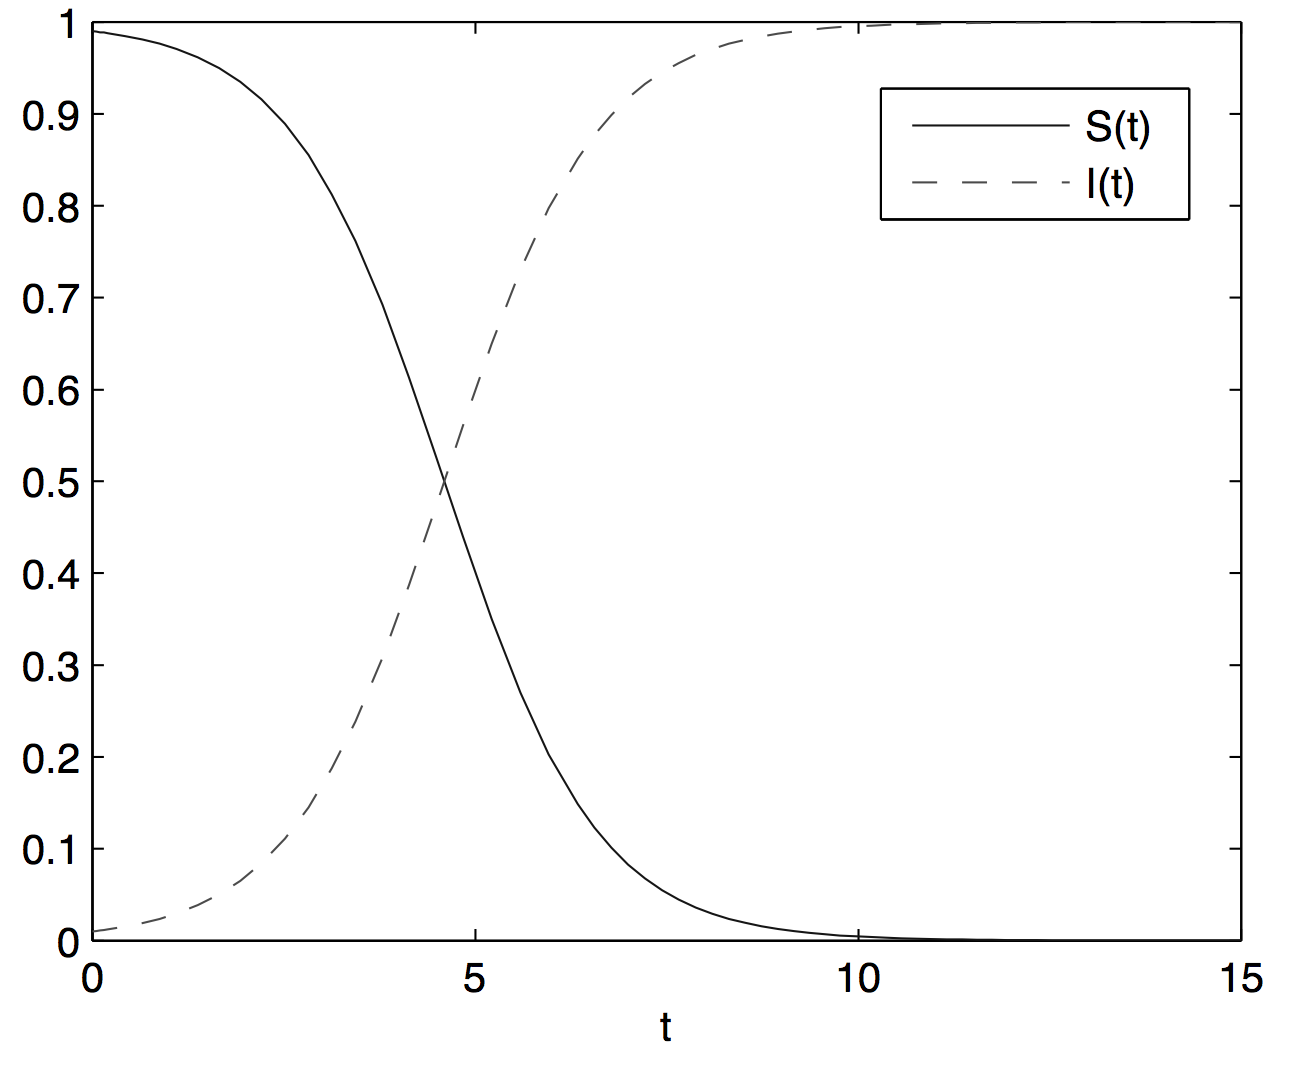
\includegraphics[width=\linewidth]{SI.png}
\end{wrapfigure}

$S(t)$: number susceptible at time $t$ \\
$I(t)$: number infected at time $t$ \\
$R(t)$: number recovered at time $t$ \\
$\beta$: differential equation parameter \\
$\gamma$: differential equation parameter

\subsubsection{SI model}

The differential equations are:
$$ \frac{dS(t)}{dt} = -\beta S(t) I(t) $$
$$ \frac{dI(t)}{dt} = \beta S(t) I(t) $$
And the normalization equation is:
$$ S(t) + I(t) = 1 $$
The closed-form solutions are logistic functions:
$$ I(t) = \frac{I(0)e^{\beta t}}{S(0) + I(0)e^{\beta t}} $$
$$ S(t) = 1 - I(t) $$
We can approximate logistic functions as exponential functions for small $t$ values.

\subsubsection{SIS model}

\begin{wrapfigure}[15]{r}[0.5in]{0.35\textwidth}
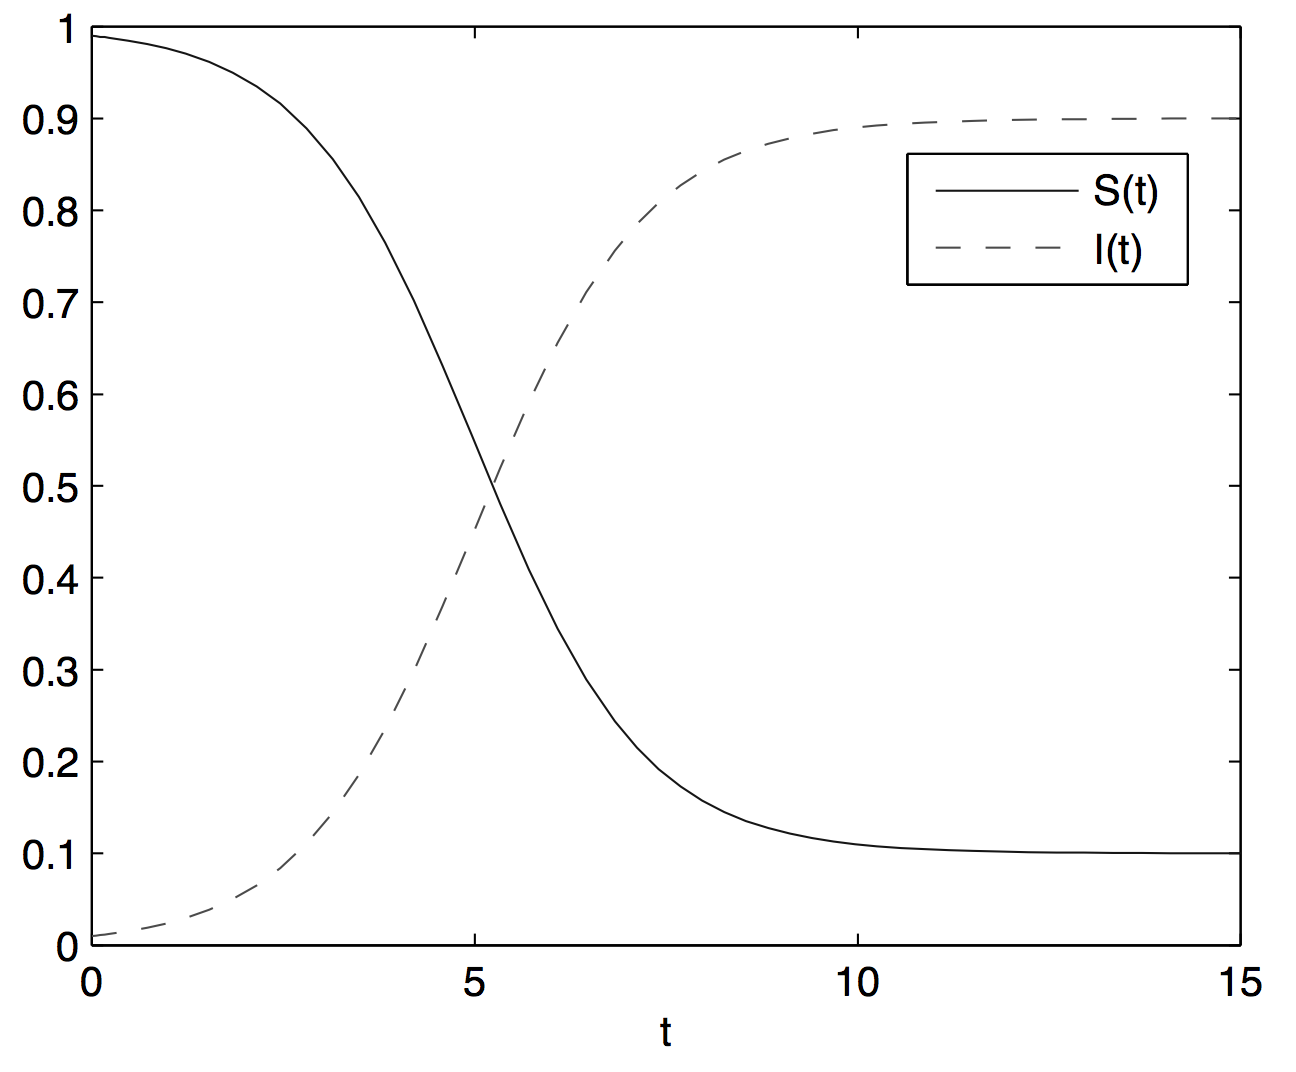
\includegraphics[width=\linewidth]{SIS.png}
\end{wrapfigure}

$$\frac{dS(t)}{dt} = \gamma I(t) - \beta S(t) I(t) $$
$$ \frac{dI(t)}{dt} = \beta S(t) I(t) - \gamma I(t) $$
And the normalization equation is:
$$ S(t) + I(t) = 1 $$
The closed-form solutions are logistic functions:
$$ I(t) = (1-\gamma/\beta)\frac{ce^{\beta t}}{1 + ce^{(\beta - \gamma) t}} $$
$$ S(t) = 1 - I(t) $$
If $\beta < \gamma$, I(t) depletes exponentially \\
If $\beta > \gamma$, I(t) goes up, but not to 100\% since some of the infected population will be going back to susceptible \\
The exact saturation percentage of I(t) depends on $\sigma = \beta/\gamma$, the \textbf{basic reproduction number}. \\
The formula is: $\text{Saturation level} = 1-\gamma/\beta = 1-1/\sigma$

\subsubsection{SIR model}

\begin{wrapfigure}[15]{r}[0.5in]{0.35\textwidth}
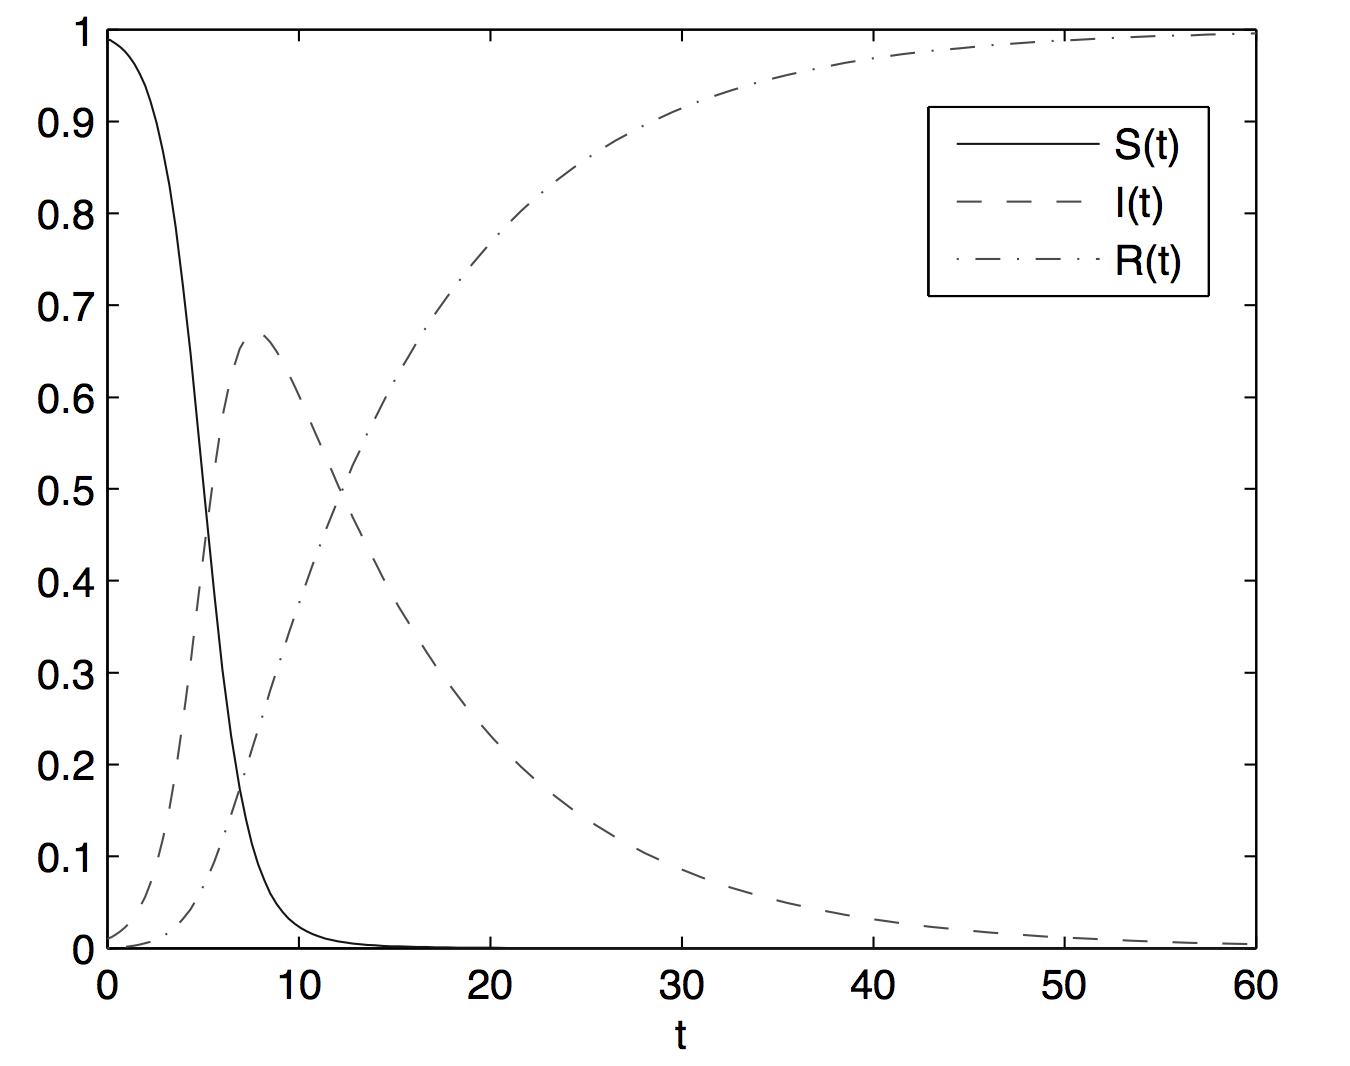
\includegraphics[width=\linewidth]{SIR.png}
\end{wrapfigure}

$$\frac{dS(t)}{dt} = \gamma I(t) - \beta S(t) I(t) $$
$$ \frac{dI(t)}{dt} = \beta S(t) I(t) - \gamma I(t) $$
$$ \frac{dR(t)}{dt} = \gamma I(t) $$
And the normalization equation is:
$$ S(t) + I(t) + R(t) = 1 $$
No closed-form solution exists to these differential equations. However:
\begin{itemize}
\item If $\sigma S(0) \leq 1$, then $I(t)$ decreases to 0 as $t \to \infty$. The initial value $S(0)$ is not large enough to create an epidemic.
\item If $\sigma S(0) > 1$, then $I(t)$ increases to a maximum of
$$I_{max} = I(0) + S(0) - 1/\sigma - \text{log}(\sigma S(0))/\sigma$$
then decreases to 0 as $t \to \infty$. This is the typical curve of an \textbf{epidemic outbreak}.
\item S(t) is always a decreasing function. The limit $S(\infty)$ as $t \to \infty$ is the unique
root in the range $(0, 1/\sigma)$ of the following equation: 
$$I(0)+S(0)−S(\infty)+ \frac{1}{\sigma} \text{log} S(\infty) =0$$
Can approximate $\sigma$ as:
$$ \sigma = \frac{\text{log}(S(0)/S(\infty))}{S(0)-S(\infty)} $$
Herd immunity occurs when $S(0) < 1/\sigma$ or $R(0) > 1 - 1/\sigma$
\end{itemize}

\subsection{Immunization strategies}

\begin{itemize}
\item Pick nodes at random (inefficient)
\item Pick high degree nodes (needs global information)
\item Acquaintance immunization: for $i = 1$ to $k$, pick random node $u$ and immunize random neighbor of $u$
\end{itemize}

\subsection{Maximizing spread of influence}

\begin{itemize}
\item Linear Threshold Model: Based on link weights $b_{u,v}$, node $u$ becomes active if sum of link weights to active nodes is higher than threshold
\item Independent Cascade Model: Based on link probabilities $p_{u,v}$, when node $u$ becomes active it gets one shot to activate each neighbor $v$ (success governed by $p_{u,v}$)
\end{itemize}

\subsection{Possible question types}

\begin{enumerate}
\item Given a graph G, compute the [degree/eigenvector/closeness/betweenness] centrality for [node/link] $i$. \\
\textit{Answer: use the definition of the given type of centrality}
\item Given a graph G, compute the diameter. \\
\textit{Answer: compute the longest shortest path length}
\item Verify that the closed-form equations for [SI/SIS/SIR] model are solutions to their corresponding differential equations. \\
\textit{Answer: differentiate the closed-form equations and plug in}
\end{enumerate}

\section{Can I really reach anyone in six steps?}

\subsection{Definitions}

\textbf{Homophily:} phenomenon of people who are alike tending to form social links \\
\textbf{Clustering coefficient:} used to quantify homophily \\
\textbf{Small world:} graph where median shortest path length grows at a rate on the order of the log of the number of nodes \\
\textbf{Poisson random graph:} a graph with a set of $n$ nodes, and for each pair of nodes decide with probability $p$ that there is a link between them (this is the \textbf{Erdos-Renyi model}) \\
\textbf{Regular graph:} a graph where every vertex has the same number of neighbors \\
\textbf{Watts-Strogatz model:} adds random (possibly long-range) links to a regular ring graph (technically replaces existing ones in the original graph)---combines elements of random graph and regular ring graph to get both the large clustering coefficient $C$ and a small expected shortest distance $L$ that grows at a rate of $\text{log}(n)$ (small world). This works because path length is an \textit{extremal property} while the clustering coefficient is an \textit{average property} \\
\textbf{Kleinberg model:} built on k-dim grid (with inherited distance), like Watts-Strogatz model but probability of having random link of length $r$ is proportional to $r^{-\alpha}$

\subsection{Variables}

$n$: number of nodes in the graph \\
$c$: expected degree of a node \\
$p$: probability that there is a link between two nodes in a random graph \\
$r$: length of random link \\
$\alpha$: Kleinberg model length parameter
$l$: longest shortest path length in the network

\subsection{Equations}

The general formula for the clustering coefficient is:
$$ C = \frac{\text{Number of triangles}}{\text{Number of connected triples}/3} \leq 1 $$ \\
In a random graph, the expected value of the clustering coefficient is:
$$ C = p = \frac{c}{n-1} $$
Also for a random graph:
$$ \text{Average path length} \propto \text{log}(n) / \text{log}(pn) $$
So you have the small world effect, but a low clustering coefficient. \\
\\
In a regular ring topology:
$$ C = \frac{3(c-2)}{4(c-1)} $$
So when $c = 2$, $C = 0$. Also, when $c$ gets large, $C \to \frac{3}{4}$ (which is much higher than $C$ in a random graph). \\
\\
For the \textbf{Kleinberg model}: \\
Probability of having random link of length: $P \propto r^{-\alpha}$ \\
$\alpha = 1$: greedy social search gives $\text{path length} \propto \text{log}^2(n)$ \\
$\alpha \neq 1$: greedy social search gives $\text{path length} > \text{poly}(n)$ \\
For $k$-dim grids (not 1-dim rings), need $\alpha = k$ instead of $\alpha = 1$.
\textit{Intuition:} In k-dim space, draw spheres with radius ($r$, $2r$, ...) around any given node. The number of nodes in the space between a radius-$r$ sphere and a radius-$2r$ sphere is proportional to $rk$. But according to the Kleinberg model, the probability of having a link to one of those nodes also drops as $rk$. These two terms cancel each other out, and the probability of having some connection $d$ hops away becomes independent of $d$. This independence turns out to give us the desired \textbf{searchability} as a function of $n$: $l$ grows no faster than a polynomial function of $\text{log}(n)$.

\subsection{Possible question types}

\begin{enumerate}
\item Given an arbitrary graph, compute the diameter, clustering coefficient $C$, and the average shortest path $L$ for the graph. \\
\textit{Answer: use $ C = \frac{\text{Number of triangles}}{\text{Number of connected triples}/3} $, and then compute the shortest path length of all paths and divide by the number of shortest paths.}
\item Generalize the clustering coefficient to clique sizes of $n$.
\textit{Answer: depends on how exactly the clustering coefficient is defined, but ensure that $ C(n\text{-clique}) = 1$ to normalize the equation}
\item What is the clustering coefficient of a ring graph with given $c$ and some large $n$? What happens if $c$ is 2? What if we let $c \to (n-1)$? \\
\textit{Answer: ignore $n$ (all we need is the fact that it is large). $ C = \frac{3(c-2)}{4(c-1)} $. When $c = 2$, $C = 0$. When $c$ gets large, $C \to \frac{3}{4}$ }
\end{enumerate}

\section{Does the Internet have an Achilles' heel?}

\subsection{Definitions}

\begin{wrapfigure}[8]{r}[0.5in]{0.35\textwidth}
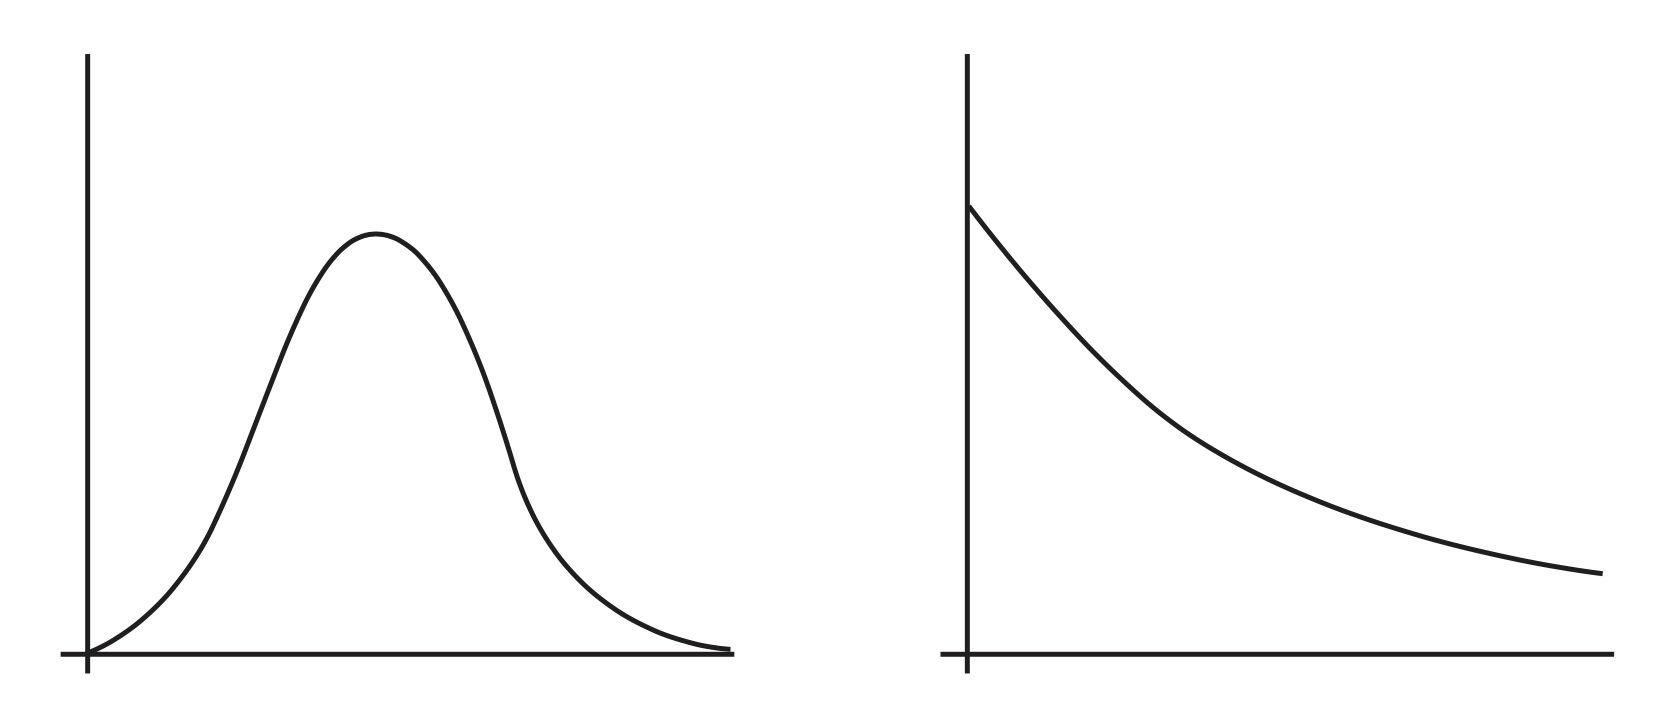
\includegraphics[width=\linewidth]{power_law.png}
\end{wrapfigure}

\textbf{Homogeneous network:} network in which degrees of nodes are similar (see first graph on the right) \\
\textbf{Long-tail distribution:} no characteristic scale in the distribution of node degrees (see second graph on the right), resulting in a \textbf{scale-free network} which is \textbf{inhomogeneous}, linear on a log-log plot
$$ \text{Prob}[X \geq x] \approx kx^{-\alpha} $$
\textbf{Zipf's Law:} $i^{th}$ most common item in set appears with
frequency proportional to $(1/i)$

\subsection{Achilles' heel argument and counterargument}

The argument that internet has an Achilles' heel uses the following facts:
\begin{itemize}
\item Scale-free networks are robust to random errors
\item But they have highly central nodes that are critical to the connectedness of the network, which are the Achilles' heel
\item Internet graph follows a power-law distribution
\end{itemize}
The internet does not have an Achilles' heel. The argument above has the following flaws:
\begin{enumerate}
\item Incomplete measurements skew the data
\item A power-law degree distribution does not imply preferential attachment
\item Functional protection sits on top of topological properties and the question of
robustness of the Internet has as much to do with protocols as with graphs
\end{enumerate}
Highly connected core nodes are rare in the internet because they would bottleneck performance of the network. This was the reason the routing protocols were designed as they are.

\subsection{Preferential attachment}

$D_i$: in-degree of node $i$ \\
$N$: existing number of nodes \\
\\
For the preferential attachment model, introduce nodes sequentially and for each node $i$ added:
\begin{itemize}
\item With probability $\theta$, connect to existing node $j$ with probability $\propto$ in-degree of node $j$:
$$\text{Prob(node } i \text{ connecting to node } j) = \frac{D_j}{\sum_k D_k}$$
\item With prob $1 - \theta$, connect to random node:
$$\text{Prob(node } i \text{ connecting to node } j) = \frac{1}{N}$$
\end{itemize}
Preferential attachment generates a scale-free degree distribution.

\subsection{Hyperbolic plane}

Use ``thin-triangle condition" as measure of network curvature: smallest side, radius of inscribed circle \\
The internet has negative curvature in the hyperbolic plane \\
Suppose each node wants to connect to every other node:
\begin{itemize}
\item In regular grid, max congestion scales as $n^{1.5}$
\item In negatively curved graph, max congestion scales as $n^2$
\end{itemize}

\begin{figure}
\centering
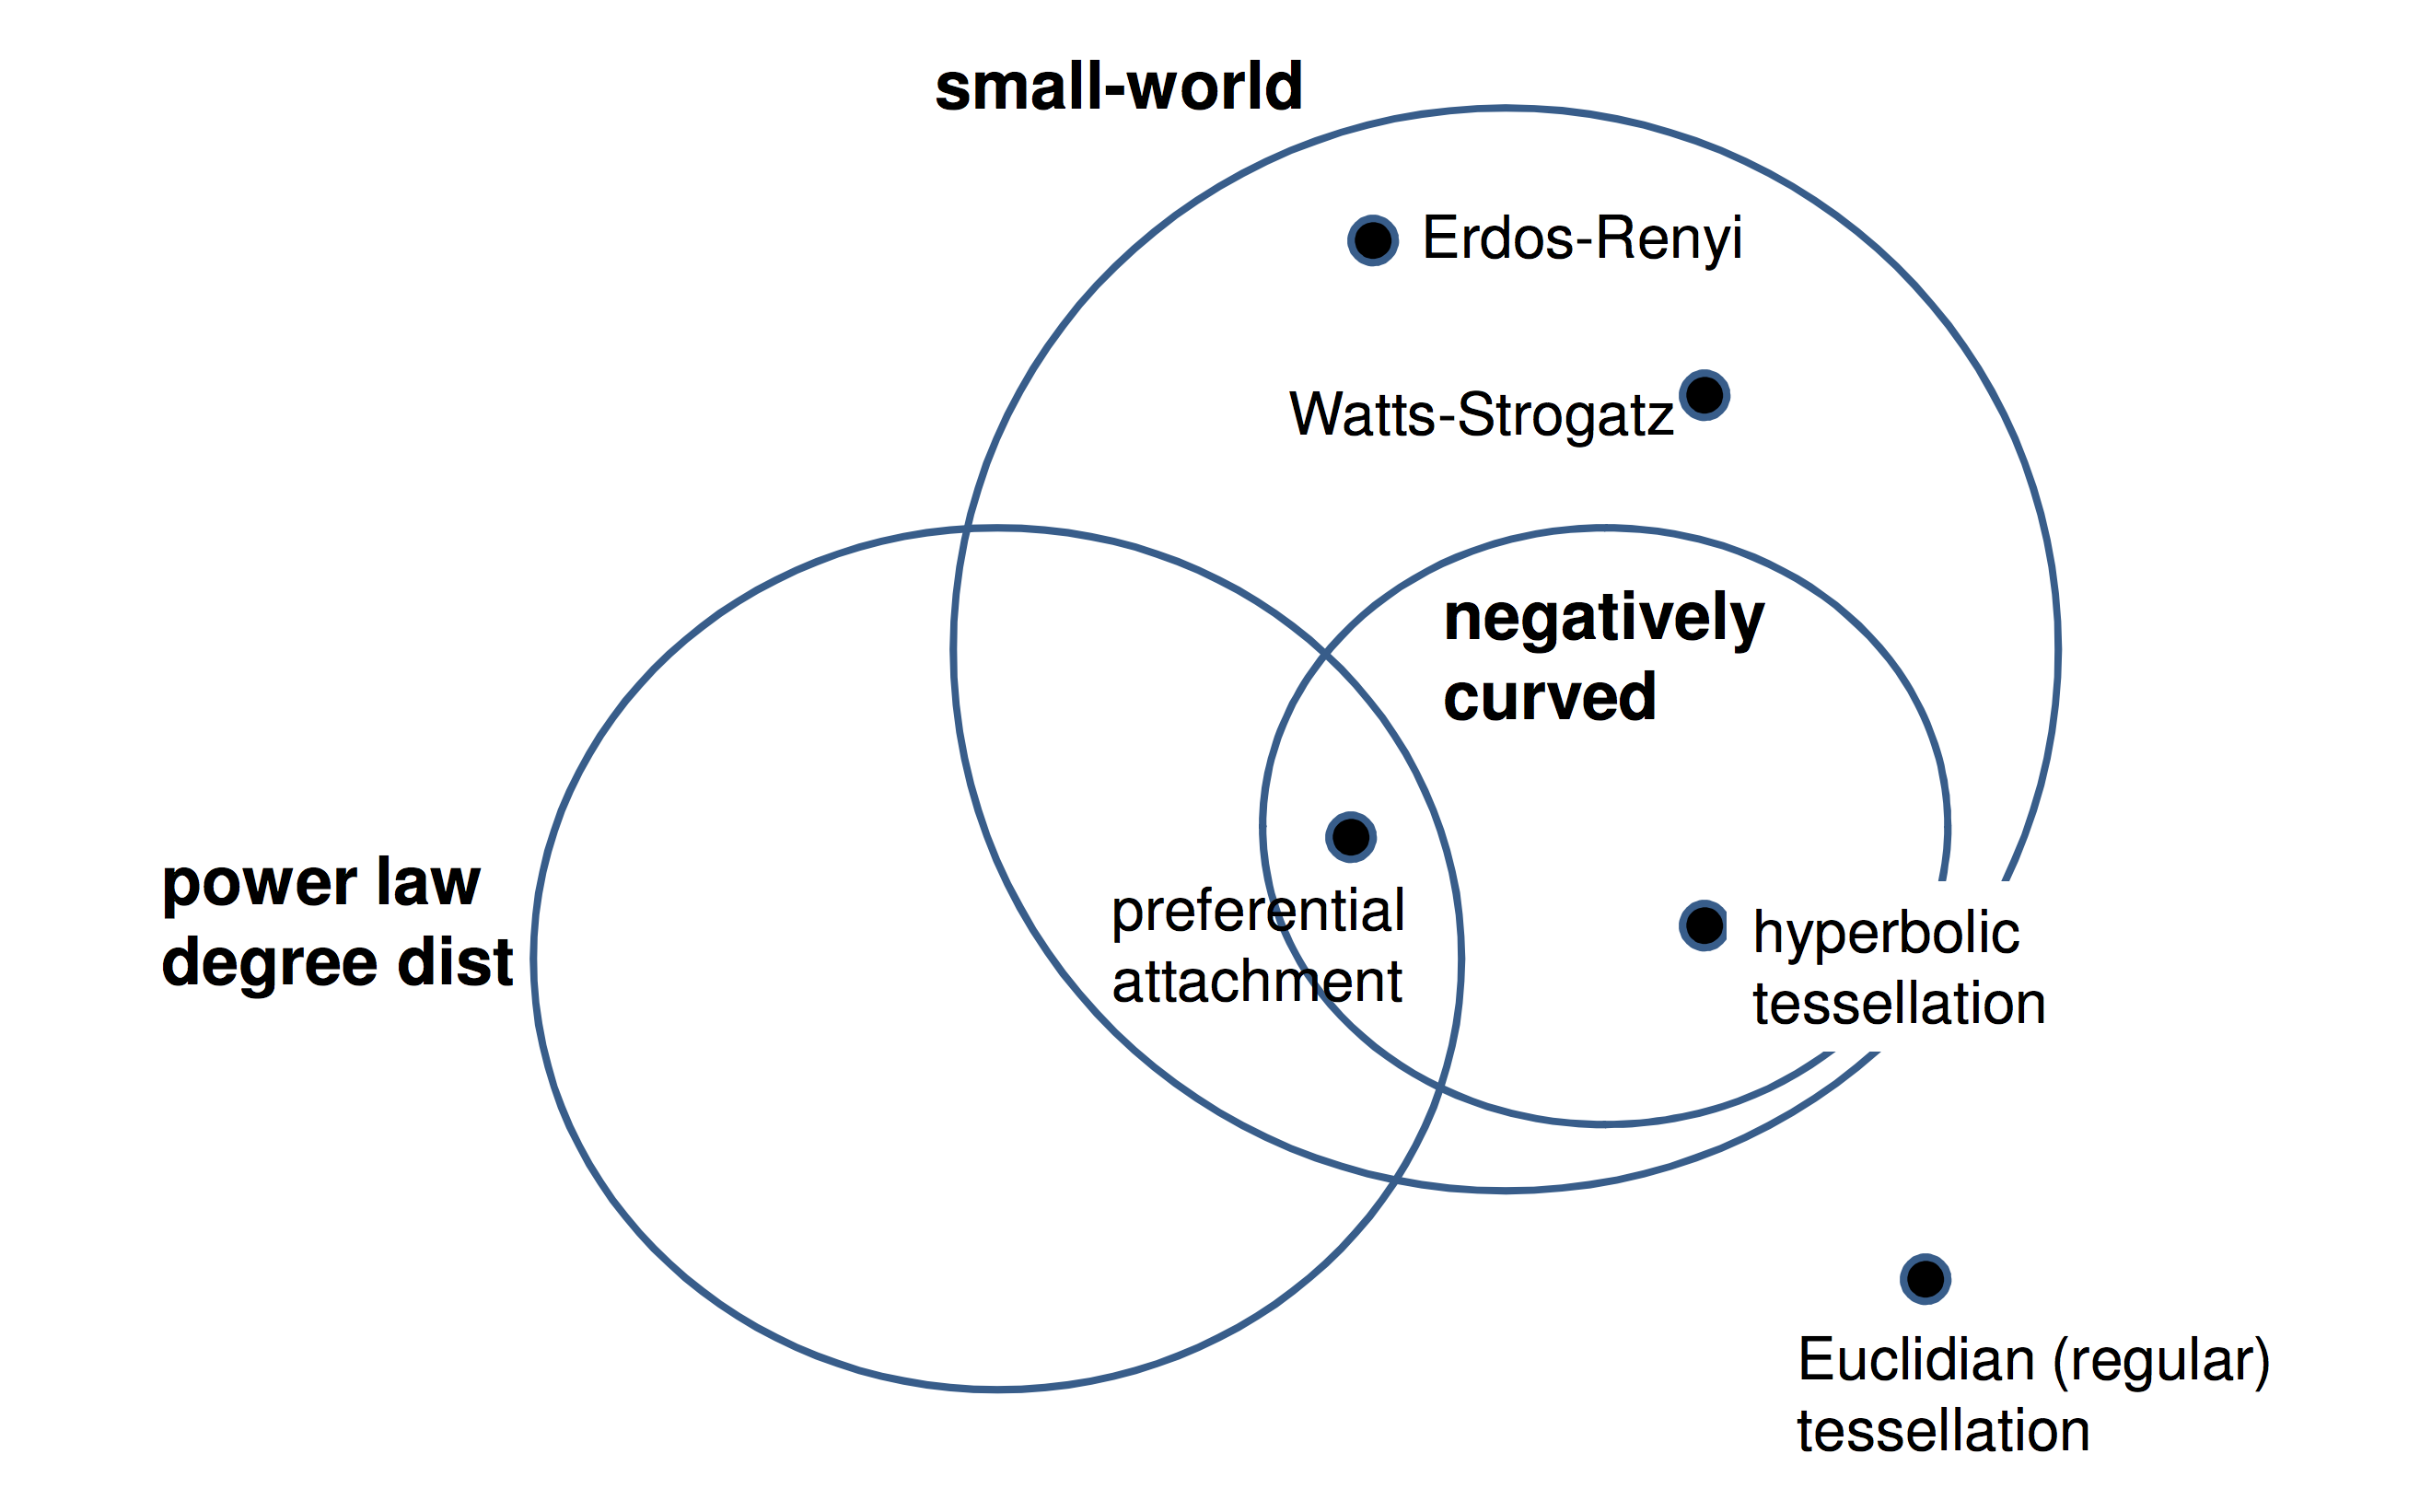
\includegraphics[width=0.98\textwidth]{graph_classification.png}
\end{figure}

\subsection{Possible question types}

\begin{enumerate}
\item Plot the approximate shape of the probability distribution of degree in a scale-free network with given $k$ and $\alpha$. Plot the approximate shape of the probability distribution on a log-log scale. Give a simple expression for the slope of the log-log scale curve. \\
\textit{Answer: the shape of the probability distribution will look like the first plot at the top of the previous page, on a log-log scale it will just have the form of a linearly decreasing function with slope $-\alpha$}
\item Suppose there are $10^5$ words in a language. Assuming Zipf's Law is true, what is the frequency of the 5th most used word? You may approximate sums using integrals where necessary. \\
\textit{Answer: get normalized frequency by doing $5^{-1}/\sum_{i=1}^{10^5} (1/i) \approx 5^{-1}/\int_{1}^{10^5} (1/i) di = 0.2/(\text{log}(10^5) - \text{log}(1)) = 0.2/5 = 0.04 $}
\item Why does the internet not have Achilles' heel? \\
\textit{Answer: make the same arguments given in the page above}
\item Suppose we are considering the preferential attachment model of some given graph with $n$ nodes. We let $\theta$ be the preferential attachment model parameter. Suppose node $i$ has in-degree $D_i$ and there are $D_{tot}$ links in the network. What is the probability that the next node we add will attach to node $i$? \\
\textit{Answer: $\theta(D_i/D_{tot}) + (1-\theta)(1/n)$} \\
NOTE: This type of problem may ask for recurrence relations to generalize the probability in one case
\end{enumerate}

\section{Why do AT\&T and Verizon Wireless charge me \$10 a GB?}

\subsection{Net neutrality debate}

Three layers to the debate:
\begin{itemize}
\item \textit{Access/Choice:} Consumers should have access to all the services offered over the Internet, and a choice of how they consume capacity on the Internet
\item \textit{Competition/no monopoly:} ISPs should have no monopoly power and the marketplace needs to have sufficient competition
\item \textit{Equality/no discrimination:} All traffic and all users should be treated the same. This may actually contradict the requirement of access/choice
\end{itemize}
There are four types of no discrimination:
\begin{itemize}
\item \textit{Service limitation:} Because of vertical integration, an ISP also becomes a content owner, possibly blocking access to other content---or an ISP could block access to voice-call apps on iPhones in order to generate more revenue for its own voice business
\item \textit{Protocol-based discrimination:} Certain protocols generate a significant amount of heavy traffic, e.g., BitTorrent, and get blocked
\item \textit{Differentiation of consumer behaviors:} Usage pricing is one of the simplest ways to correlate pricing with consumer behavior; if consumer A takes up more capacity, she pays more
\item \textit{Traffic management and QoS provisioning:} Examples include maintaining more than one queue in a router, scheduling traffic with weighted fair queuing, or prioritizing emergency traffic like healthcare-monitor signals over non-essential software updates
\end{itemize}
Neutrality against service limitations is essential, neutrality against protocol-discrimination is debatable, neutrality against consumer behavior differentiation is harmful, and neutrality against traffic management is impossible

\subsection{Definitions}

\textbf{Social welfare maximization:} maximizing the sum of utilities across all users \\
\textbf{Net utility maximization:} a user picks the $x$ that maximizes the difference between utility and price paid \\
\textbf{Demand elasticity:} normalized price sensitivity of demand \\
\textbf{Diminishing marginal returns:} utility functions eventually become concave, and even possibly flat, for sufficiently large x \\
\textbf{Tragedy of the commons:} want to internalize the external effects on others. 
To fix, change the net utility calculation of each person from $\text{maximize}[U(x) - x]$ to $\text{maximize}[U(x) - Nx]$. \\
\textbf{ISP Monopoly:} the ISP can try to push the user's net utility to 0 \\
\textbf{Bertrand Competition Model:} two operators have same cost then competition makes them have 0 profit (this is the \textbf{Bertrand curse}, solution is to differentiate products)

\subsection{Variables}

$x_i$: some performance metric like throughput for session $i$ \\
$U_i(x_i)$: utility function of session $i$ \\
$p_i$: unit price for session $i$ \\
$D_i$: the demand function of session $i$ \\
$\eta_i$: the demand elasticity of session $i$
$\alpha$: fairness parameter \\
$N$: number of people \\
$C_j$: data cap

\subsection{Net utility maximization}

In \textbf{net utility maximization:}
$$ \text{argmax}_x[U(x) - px)] $$
$$ U'(x) = p $$
$$ x = U'^{-1}(p) = D(p) $$
Thus the demand elasticity is:
$$ \eta = -\frac{\partial D(p)/\partial p}{D(p)/p} $$
If utility is logarithmic, then the demand function is $x = 1/p$ and the elasticity is 1. \\
\\
Company profit is given by:
$$ P(p) = (p - c)D(p) $$
Users should choose their data caps $C_j$ to maximize their expected surplus:
$$ \sum_i \left(U_i(C_j) - r(C_j)\right)*\text{Prob}[U(.) = U_i(.)] $$

\subsection{$\alpha$-fair utility functions}

\textbf{$\alpha$-fairness} of $\MatrixVariable{x}$ is defined by the following condition:
$$ \sum_i \frac{x_i - y_i}{x_i^\alpha} \leq 0 $$
That means, roughly speaking, that the (normalized) deviation from x does not pay off. \\
The following utility function is $\alpha$-fair:
$$ U_\alpha(x) = \begin{cases} x^{1-\alpha}/(1-\alpha) & \alpha \neq 1 \\ \text{log}(x) & \alpha = 1 \end{cases} $$
Smaller $\alpha$ means more elastic demand:
\begin{itemize}
\item $\alpha = 0$ simply maximizes the sum of resources, is often unfair because some user $i$ may receive 0 resource
\item $\alpha = 1$ is called \textbf{proportional fairness}
\item $\alpha \to \infty$ is called \textbf{max-min fairness}---cannot increase some $x_i$ without reducing some other $x_j$ that is already smaller than $x_i$
\end{itemize}

\subsection{Possible question types}

\begin{enumerate}
\item What is your take on the net neutrality debate? \\
\textit{Answer: open-ended, but consider layers of the debate and types of discrimination}
\item Given a utility function $U(x)$ and pricing function $p(x)$, compute the demand function $D(p)$ and the demand elasticity $\eta$. \\
\textit{Answer: use $x = U'^{-1}(p) = D(p)$ and $\eta = -\frac{\partial D(p)/\partial p}{D(p)/p}$}
\item With the result from above: if we have a monopoly ISP, express one given parameter in terms of the others. \\
\textit{Answer: in a monopoly, just minimize user's net utility by setting U(x) = p(x) and then solve the system of equations}
\item Suppose now that there is a competing ISP. Why would this be a problem for the ISPs? What is a good solution? \\
\textit{Answer: problem is the Bertrand curse, solution is to differentiate products}
\item What kind of fairness does $U(x) \propto \text{log}(x)$ achieve?
\textit{Answer: proportional fairness, since it is $U_\alpha$ with $\alpha = 1$}
\item Make a rough sketch of the plot of $U_\alpha(x)$ for $\alpha = 0, 0.5, 1, 2, \infty$. \\
\textit{Answer: plot $U_\alpha(x) = \begin{cases} x^{1-\alpha}/(1-\alpha) & \alpha \neq 1 \\ \text{log}(x) & \alpha = 1 \end{cases}$}
\item Determine the profit function of a company as a function of price, given its demand function and cost function. Plot it. \\
\textit{Answer: use $P(p) = (p - c)D(p)$ and plot the function}
\item Find the price that maximizes the profit $P(p)$ of the company. \\
\textit{Answer: differentiate $P(p)$ and set to 0, then solve for p}
\end{enumerate}

\section{How can I pay less for each GB?}

\subsection{Definitions}

\textbf{Smart Data Pricing (SDP):} how to price data in an intelligent manner, examples include hourly-rate model, expected-capacity pricing, priority pricing, two-sided pricing, location-dependent pricing, time-dependent pricing \\
\textbf{Win-win situation:} ISPs generate more revenue, lowers cost, and reduces churn; consumers pay less per GB of data; content providers attract more eyeballs; vendors sell more innovative software and hardware

\subsection{Variables}

$p$: reward offered for waiting a time $t$ \\
$w(p,t)$: waiting function \\
$\beta$: parameter of waiting function that specifies how users' willingness to shift their traffic falls off with time

\subsection{Equations}
 
The \textbf{waiting function} tells us the likelihood a user is willing to shift traffic by an amount $t$ for a reward $p$. A common example is:
$$ w(p,t) = \frac{p}{(t+1)^\beta} $$

\subsection{Sponsoring content}

$T$: traffic before sponsoring (in bytes) \\
$(1+y)T$: traffic after sponsoring \\
$pyT$: additional profit due to sponsoring \\
$\gamma(1+y)T$: cost of sponsoring \\
\\
Sponsoring only makes sense if:
$$ pyT > \gamma(1+y)T $$

\subsection{Possible question types}

\begin{enumerate}
\item Suppose before TDP, we have a given volume of traffic during the day and night for two different kinds of traffic A and B. Let $\rho$ be the amount charged to the user per unit volume, $p_n$ be the reward during the night, and $p_d$ be the reward during the day. Suppose we are also given the probability function of shifting traffic from day to night $w_{D \to N}$ and vice versa $w_{N \to D}$ for A and B. Let the company pays $Y$ per unit volume for going over maximum capacity $M$. Compute the optimal values of $p_n$ and $p_d$. How much should the companies subsidize daytime traffic and nighttime traffic? \\
\textit{Answer:
$$ C_r = \text{Cost of offering rewards} = w_{D \to N} \sum_{A,B} [\text{traffic D} \to \text{N}] + w_{N \to D} \sum_{A,B} [\text{traffic N} \to \text{D}] $$
$$ C_c = \text{Cost of exceeding capacity} = Y \left( \sum_{day, night} \sum_{A,B} max(0,[\text{traffic shifted to other time of day}] - M) \right) $$
Then to get $p_n$ and $p_d$:
$$ \text{minimize}_{p_n, p_d}[C_r + C_c] $$
You can do the above using a simple plot. Then just subsidize by amount $p_n \rho$ during night and $p_d \rho$ during day.
}
\item Given $T$, $y$, $p$, $\gamma$, does it make sense for a company to sponsor its content? \\
\textit{Answer: only if $pyT > \gamma(1+y)T$}
\end{enumerate}

\section{How does traffic get through the internet?}

\subsection{Packet switching}

Advantages are (1) ease of connectivity and (2) scalability due to efficiency\\
\\
\textbf{Statistical multiplexing:} packet switching can flexibly map demand of capacity onto supply of capacity, helps with bursty traffic, no resources occupied by idle hosts \\
\textbf{Resource pooling:} putting resources into a single pool lowers the chance that some demand must be turned down because one set of resources is fully utilized

\subsection{Protocol layers}

\begin{enumerate}
\item \textbf{Physical layer:} convert information into ``physics" i.e. light, electricity, radiation etc.
\item \textbf{Link layer:} send to correct next hop, local retransmission, local coding, local scheduling, congestion management
\item \textbf{Network layer:} send to correct destination
\item \textbf{Transport layer:} end-to-end retransmission, end-to-end coding, global congestion management
\item \textbf{Application layer:} what information to send
\end{enumerate}

\subsection{Definitions}

\textbf{End-to-end principle:} end hosts are intelligent, middle of network is dumb \\
\textbf{Thin waist:} network and transport layers (TCP/IP) have been remarkably consistent over time as physical layers and application layers get upgrades \\
\textbf{Software-Defined Networking (SDN):} do routing computations in a smart centralized manner

\subsection{Routing Information Protocol (RIP)}

Is an implementation of \textbf{Bellman-Ford algorithm} for shortest paths \\
Bellman-Ford algorithm works as long as there are no negatively weighted cycles \\
Initialize with:
$$ p_i[0] = \infty \; \; \forall i $$
Then iterate the following line for all $i$ until there are no updates to $p_i$:
$$ p_i[t + 1] = \underset{k \in O(i)}{\text{min}} \lbrace c_{ik} + p_k[t] \rbrace \; \; \forall i $$
You only need to store destination, cost, and next node.

\subsection{IP and CIDR blocks}

\begin{itemize}
\item IP addresses are four 8-bit numbers (0-255) ranging from 0.0.0.0-255.255.255.255 \\
\item CIDR blocks are a way of specifying IP address ranges by making certain bits variable \\
\item ``xxx.xxx.xxx.xxx/24" would mean that the first 24 bits are fully specified and the rest (the other 8) can be matched with any binary string \\
\item \textbf{Longest prefix match:} match entry with longest prefix
\end{itemize}

\subsection{Possible question types}

\begin{enumerate}
\item Simulate RIP on a given graph. \\
\textit{Answer: use $p_i[0] = \infty \; \; \forall i$ and $p_i[t + 1] = \underset{k \in O(i)}{\text{min}} \lbrace c_{ik} + p_k[t] \rbrace \; \; \forall i$ }
\item Will you get the count-to-infinity problem if link $l$ breaks? What is one way you could solve this problem if it occurred in your network? \\
\textit{Answer: simulate RIP for a few more steps to see if it happens; one implementation would be to set a threshold so that once a cost to a node reaches this threshold, a link is assumed to be broken to that node}
\end{enumerate}

\section{Why doesn't the Internet collapse under congestion?}

\subsection{TCP Reno}

Estimate packet loss and delay by trying to estimate the normal (minimum) round trip time (RTT) between the sender and the receiver and using this as a baseline to see how congested the link is. RTT is a result of \textbf{propagation delay} and \textbf{queueing delay}. TCP Reno only uses loss as a feedback signal, but delay is actually better since it has more information. \\
\\
Each sender maintains a sliding window called the \textbf{congestion window}, $cwnd$. TCP Reno uses \textbf{Additive Increase Multiplicative Decrease (AIMD)}---if all the cwnd outstanding packets are received at the receiver properly (i.e., in time and not out of order more than twice), increase the $cwnd$ by 1 each RTT, otherwise, decrease it by cutting it in half. \\
\\
The TCP Reno utility function is given by:
$$ U_i(x_i) = \frac{\sqrt{2}}{d_i} \text{arctan} \left( \sqrt{\frac{1}{2}} x_i d_i \right) $$

\subsection{Variables}

$U_i(x_i)$: utility function of host $i$ \\
$x_i$: send rate of host $i$ \\
$R_{li}$: binary-valued indicator, so that $R_{li} = 1$ if source $i$'s session traverses link $l$, and $R_li = 0$ otherwise \\
$c_l$: capacity of link $l$ \\
$p_l$: path price of link $l$ \\
$q_l$: link price of $l$ \\
$y_l$: total load on link $l$ \\
$\beta$: \textbf{stepsize}, controls trade-off between a convergence guarantee and the convergence speed

\subsection{Network Utility Maximization (NUM)}

$$ \text{maximize } \sum_i U_i(x_i) $$
$$ \text{subject to } \MatrixVariable{R}\MatrixVariable{x} \leq \MatrixVariable{c} $$
$$ \text{variables } x_i \geq 0 \; \; \forall i $$
\\
This problem can be solved distributively:
$$ q_i = \sum_{l \in L(i)} p_l \; \; \forall i $$
$$ x_i[t] = D_i(q_i[t]) = U_i'^{-1}(q_i[t]) \; \; \forall i $$
$$ y_l[t] = \sum_{i \in S(l)} x_i[t] $$
$$ p_l[t] = \text{max}(0, p_l[t-1] + \beta(y_l[t] - c_l)) \; \; \forall l  $$


\subsection{Possible question types}

\begin{enumerate}
\item Suppose we had a link in which packets are dropped when there are more than $n$ in the queue. Assuming our host is the only one using a link, plot the qualitative shape of the $cwnd$ over time. What is one problem with having this kind of shape? \\
\textit{Answer: graph looks like a sawtooth, starts from 0 increasing to $n$ then decreasing to $n/2$; this shape is not great because there is lots of variation in the transmission rate (high jitter).}
\item Given a utility function, a graph of links and connections, the capacity of each link, and some starting values, simulate NUM with given $\beta$. What will the rates $x_i$ converge to? \\
\textit{Answer: $R_{li}$ can be inferred from the graph, follow the distributed algorithm to update over the iterations; to find out the convergence, look at the fairness of the utility function; if it is proportional fair, $x_i$ will be proportional to then inverse of the links traversed} \\
NOTE: other types of questions will be similar to those in Chapter 11.
\end{enumerate}

\section{How should ridesharing platforms balance supply and demand? (Q24 in lecture slides)}

\subsection{Static Pricing}

\begin{itemize}
\item Simpler model
\item Uses a fixed price for all times
\item Important to get this fixed price right
\end{itemize}

\subsection{Dynamic Pricing}

\begin{itemize}
\item More complicated model
\item Uses a different price to balance supply and demand
\item Less important to get the price exactly right ahead of time
\item Robust to parameter uncertainty
\end{itemize}

\subsection{Possible question types}

\begin{enumerate}
\item What are the differences between static and dynamic pricing? Give advantages and disadvantages of each. \\
\textit{Answer: see above}
\end{enumerate}

\section{What's inside the cloud of iCloud?}

\subsection{Advantages of cloud computing}

\begin{itemize}
\item To the cloud users, the key benefit is \textbf{resource pooling}
\item To the cloud providers, the benefits are economies of scale and smoothing of burstiness across more users
\end{itemize}

\subsection{Metrics for interconnection topology}

\begin{itemize}
\item Worst-case pairwise end-to-end capacity
\item \textbf{Bisection bandwidth}: the capacity on all the links between two equal-sized halves of the network is called a bisection; the worst case of that over all possible combinations of halves of the network is called the bisection bandwidth
\item \textbf{Non-blocking} if any pair of (unused) input and (unused) output can be connected as each traffic session (a switching request) arrives. \textbf{Rearrangeably non-blocking} is when some existing pairs’ connection needs to be rearranged in order to achieve the non-blocking property
\end{itemize}

\subsection{Clos networks}

\textbf{Clos networks} are a type of \textbf{multi-stage switched networks}: instead of using tree structures for the topology which have single points of failure and involve scaling up the number of ports per router, Clos networks scale out the topology (which can be done to an arbitrary extent) \\
\\
Wiring within each switch determines the switching pattern. Wiring among the switches is fixed a priori by the design of the Clos network. \\
\\
3-stage Clos network is specified by $(n, m, r)$: \\
$r$ input switches ($n \times m$) \\
$r$ output switches ($m \times n$) \\
$m$ middle-stage switches ($r \times r$) \\
\\
Each of the input and output switches is connected to each of the middle-stage switches. \\
If a centralized controller decides the switching patterns: \\
$m \geq 2n - 1 \implies$ non-blocking \\
$m \geq n \implies$ rearrangeably non-blocking \\
\\
\begin{wrapfigure}[8]{r}[0.5in]{0.35\textwidth}
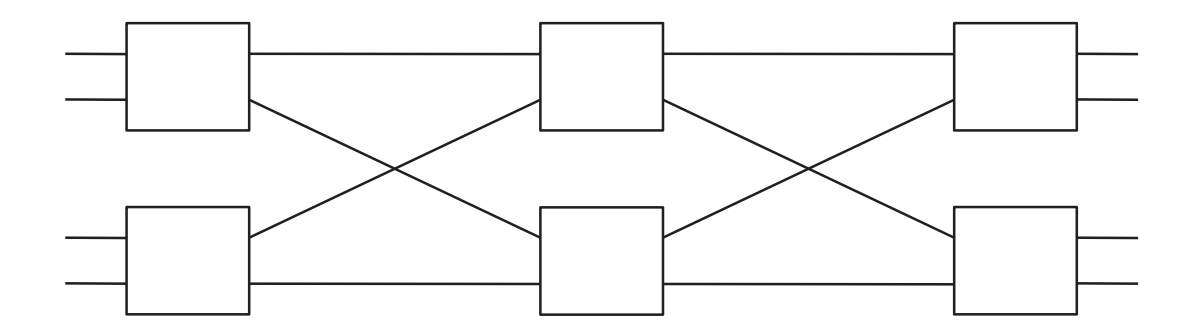
\includegraphics[width=\linewidth]{4x4as2x2.png}
\end{wrapfigure}
A \textbf{fat tree} is just a Clos network folded down the middle (since it is symmetric about the middle), has bidirectional links \\
\\
A ($4 \times 4$) switch in a Clos network can be expanded into two ($2 \times 2$) by adding 2 middle-stage switches with crossings as shown to the right. Then these expansions can be cross-linked appropriately to get the expand Clos network.

\subsection{Assignment of Jobs to Servers}

\begin{itemize}
\item Perfect load balancing: Assign each job to least loaded server
\item Random load balancing: Assign job to random server, with high probability max load on server is
$$\frac{\text{ln } n}{\text{ln ln } n(1 + O(1))} $$
\item Power of two choices: Pick two servers at random, assign to least loaded, with high probability max load on server is
$$ \frac{\text{ln ln } n}{\text{ln ln } 2} + \text{const} $$
\end{itemize}

\subsection{Possible question types}

\begin{enumerate}
\item Given a Clos network of size $(n, m, r)$ will it be non-blocking? Rearrangeably non-blocking? \\
\textit{Answer: $m \geq 2n - 1 \implies$ non-blocking, $m \geq n \implies$ rearrangeably non-blocking}
\item Given a Clos network with some high-degree routers, expand the middle routers to lower-degree routers and draw the fat tree representation of the final network layout. \\
\textit{Answer: expand the switches as described above; to fold into fat tree, just give first half of the tree and indicate bidirectionality of links}
\item Design an algorithm for routing traffic on an $(m, n, r)$ Clos network with $m \geq n$. \\
\textit{Answer: open-ended, but might want to use one of the techniques in assignment of jobs to servers; this will not deal with the case where the network is rearrangeably non-blocking but not fully non-blocking, in this case, just route middle router backwards, unplug old link and find new spot for it and iterate until every input is connected to its output (this is somewhat inefficient, but it will work)}
\end{enumerate}

\section{IPTV and Netflix: How can the Internet support video?}

\subsection{Types of video}

\begin{itemize}
\item Real-time vs precoded
\item Streaming or download
\item Channelized or on-demand
\item Unicast vs multicast vs broadcast
\end{itemize}

\subsection{UDP vs TCP}

\textbf{UDP (User Datagram Protocol)}: smaller header, no 3-way handshake, no retransmissions, no congestion management, only gives sequencing info \\
\\
TCP maintains too many states for each session compared with UDP. So UDP can support many more parallel sessions at the same time. \\
TCP header is 20 bytes and UDP is 8 bytes. For small control packets, this difference in overhead matters. \\
\textbf{Real-time Transport Protocol (RTP)} runs on top of UDP

\subsection{Compression}

\textbf{Lossless/lossy compression:} exploiting redundancies to reduce video size basically \\
\textbf{Rate-distortion tradeoff:} if you compress more, you may get distortion due to approximations

\subsection{Group of Pictures (GoP)}
\textbf{GoP} is a form of motion compensation with inter-frame prediction. There are three types of frames, and collectively a set of them form a Group of Pictures (GoP).
\begin{itemize}
\item \textbf{I frame (Intra-coded):} This is an independent frame. Its encoding does not depend on the frames before or after it. Most important.
\item \textbf{P frame (Predictive-coded):} This type of frame depends on the previous I (or P) frame, but not the one after it. Losses are tolerable.
\item \textbf{B frame (Bidirectionally predictive-coded):} This type of frame depends on both the I (or P) frames before and after it. Losses are tolerable.
\end{itemize}

\subsection{Measuring error}

Mean Squared Error:
$$ \text{MSE} = \frac{1}{mn} \sum_{i=0}^{m-1} \sum_{i=0}^{n-1} [I(i,j) - K(i,j)]^2 $$
Peak Signal to Noise Ratio:
$$ \text{PSNR} = 10 \log_{10} \left( \frac{\text{Max}^2}{\text{MSE}} \right) $$

\subsection{Recovering from frame drops}

\begin{itemize}
\item If receiver misses I-frame, display last available frame
\item If receiver misses reference frame of P-frame, display last available frame
\item If receiver misses one reference frame of B-frame, display other reference frame
\end{itemize}

\subsection{Pixel encodings}

\begin{itemize}
\item RGB \\
Red, green, blue values; bad because doesn't give contrast
\item YCbCr \\
Y is luma, Cb and Cr are blue-difference and red-difference
$$ Y = K_RR + (1-K_R-K_B)G + K_BB $$
$$ P_B = \frac{B-Y}{2(1-K_B)} $$
$$ P_R = \frac{R-Y}{2(1-K_R)} $$
$$ K_B = 0.114, \; K_R = 0.229 $$
\end{itemize}

\subsection{Latency-Jitter tradeoff}

$\MatrixVariable{V}$: transmission time \\
$\MatrixVariable{A}$: arrival time \\
$P_i$: playback time of packet $i$ \\
latency: time between playback and transmission $P_i - V_i$
$$ \text{minimize } \sum_i (P_i - V_i) $$
$$ \text{subject to } P_{i+1} = P_i + 1, \;\; P_i \geq A_i, \;\; \forall i $$
$$ \text{variables } \lbrace P_i \rbrace $$
Visual inspection solution: shift a unit step function $P$ to left, until $P_k = A_k$ for some $k$, and $P_i \geq A_i \; \forall i \neq k$. Make curve P as close to curve A as possible but still below.

\subsection{DASH optimization}

Pick video rate for each user to maximize quality, satisfy capacity constraints, minimize rate switches
$$ \underset{x_{ij}}{\text{max}} \sum_{i=1}^N \sum_{j=1}^{M_i} (u_{ij} - \alpha f_{ij}) x_{ij} $$

\subsection{Possible question types}

\begin{enumerate}
\item Given an application, would you suggest using TCP or UDP? Why? \\
\textit{Answer: if the application requires reliability, use TCP (which has handshake and retransmission), but for broadcasts, use UDP because no state is required on the server and packets have smaller headers}
\item Given a sequence of I, P, B frames, how would you recover from a given frame dropping? What would be the [MSE/PSNR]? \\
\textit{Answer: if receiver misses I-frame, display last available frame; if receiver misses reference frame of P-frame, display last available frame, if receiver misses one reference frame of B-frame, display other reference frame; then use error formulas to compute error}
\item Convert an RGB value to YCbCr. \\
\textit{Answer: use $Y = K_RR + (1-K_R-K_B)G + K_BB$, $P_B = \frac{B-Y}{2(1-K_B)}$, $P_R = \frac{R-Y}{2(1-K_R)}$, $K_B = 0.114, \; K_R = 0.229$}
\item Given transmission and arrival times, plot them and find a playback function that works and has no jitter. What is the latency? \\
\textit{Answer: plot $\MatrixVariable{V}$ and $\MatrixVariable{A}$ as step functions, make curve P as close to curve A as possible but still below and find distance between P and V to get latency} \\
NOTE: May also ask probabilistic version of this problem
\end{enumerate}

\section{Why is WiFi faster at home than at a hotspot?}

\subsection{Slotted Aloha}

\textbf{Slotted Aloha} is a simpler model than WiFi that illustrates some points.\\
\\
$n$ transmitters \\
$p$ probability of transmission in slot \\
\\
A transmission is successful if it is the only one for a given time slot
$$ \text{Avg transmissions per time slot} = p $$
$$ \text{Avg successful transmissions per time step} = p(1-p)^{n-1} $$
Average number of successful transmissions per time step is maximized when $p = 1/n$. \\
More generally, we need:
$$ \sum_i p_i = 1 $$
\\
In reality, collisions are complex and may not necessarily result in both packets/frames being dropped.\\
\\
In the case of a general graph, the problem is:
$$ \text{max } F = \sum_{(n,m) \in I} w_{nm} \log \mu_{nm} $$
$$ \mu_{nm} = p_{nm} \prod_{m \in N_k, k \neq n} (1 - p_k) $$
Solution is:
$$ p_{nm} = \frac{w_{nm}}{\sum_{(l,k) \in S_n} w_{lk}} $$

\subsection{Random exponential backoff}

$W$ is the size of the \textbf{contention window}
\begin{enumerate}
\item After successful transmission, initialize
$$ W = W_{\text{min}} $$
\item Wait for random number of slots between 0 and W, then transmit
\item If collision, double W and go to step 2
\end{enumerate}
There will also be a min and max contention window.

\subsection{Hidden node}

Receiver suffers interference but the transmitter does not know that \\
Two receivers interfere with each other but cannot detect each others presence \\
\textit{Solution:} \textbf{Request-to-Send/Clear-to-Send (RTS/CTS)} signals to communicate \\
Router sends CTS to let other hosts know that someone is trying to communicate (might be outside of their range)\\
Potential interferers stay silent for time specified by CTS

\subsection{Possible question types}

\begin{enumerate}
\item Simulate exponential backoff given a sequence of random numbers. \\
\textit{Answer: use random exponential backoff procedure above}
\item Given a graph and transmitter $A$ trying to transmit to receiver $B$, which node(s) might cause the hidden node problem? What's the solution to this problem? \\
\textit{Answer: nodes that are visible to $B$ but not $A$ might cause a problem, can fix with RTS/CTS}
\end{enumerate}
NOTE: other types of problems will involve utility functions introduced in earlier chapters

\section{Why am I getting only a few \% of the advertised 4G speed?}

\subsection{Speed reduction}

\subsubsection{Air-interface}

\begin{enumerate}
\item Propagation channel: \textbf{path loss} (signal strength drops as distance of propagation increases), \textbf{shadowing} (obstruction by objects), and multipath \textbf{fading} (signal bounces off of many objects, is collected at the receiver from multiple paths)
\item Interference: users interfere with one another, near-far problem
\end{enumerate}

\subsubsection{Backhaul network}
\begin{enumerate}
\item Link congestion (links go over-capacity)
\item Node problems (servers go over-capacity or don't work fast)
\end{enumerate}

\subsubsection{Protocols}
\begin{enumerate}
\item Protocol semantics
\item Packet headers
\item Control-plane signaling
\end{enumerate}

\subsection{Network management}

\begin{itemize}
\item Performance: Monitor, collect, analyze metrics
\item Configuration: Update control knobs in different protocols
\item Charging: Maintain data needed to identify how to charge each user
\item Fault-management: Monitor to see whether links or nodes are down, and then contain, repair, and diagnose
\item Security: Authentication, maintain integrity, check confidentiality
\end{itemize}

\subsection{Speed metrics}

Can ask: which layer, which location, when, what application? \\
\\
$W$: bandwidth \\
\textbf{Shannon rate:}
$$ \text{rate}_i = W \log_2(1 + \text{SIR}_i) $$

\subsection{Possible question types}

\begin{enumerate}
\item What is the Shannon rate at a given bandwidth and SIR vector? \\
\textit{Answer: use $\text{rate}_i = W \log_2(1 + \text{SIR}_i)$}
\end{enumerate}

\section{Is it fair that my neighbor's iPad downloads faster?}

\subsection{Possible question types}

\begin{enumerate}
\item Which kind of fairness do you think is the best? Give reasoning. \\
\textit{Answer: open-ended}
\end{enumerate}

\end{document}
